\section{ISISDLM Namespace Reference}
\label{namespaceISISDLM}\index{ISISDLM@{ISISDLM}}


\subsection*{Compounds}
\begin{CompactItemize}
\item 
struct {\bf Cube\-Dims}
\item 
class {\bf Cube\-Io\-Policy}
\item 
struct {\bf Delete\-Object}
\item 
class {\bf File\-Handler}
\item 
class {\bf File\-Repository}
\item 
class {\bf i\-File}
\item 
class {\bf Keyword\-Handler}
\item 
struct {\bf Keyword\-Handler::Key\-Spec}
\item 
class {\bf Keyword\-Handler::Pvl\-Aggregate}
\item 
class {\bf Propagation\-Handler}
\item 
struct {\bf Raw\-IO}
\item 
struct {\bf Std\-IO}
\end{CompactItemize}
\subsection*{Typedefs}
\begin{CompactItemize}
\item 
typedef {\bf Cube\-Io\-Policy}$<$ double, IDL::Idl\-Double, {\bf Std\-IO} $>$ {\bf Double\-IO}
\item 
typedef {\bf Cube\-Io\-Policy}$<$ unsigned char, IDL::Idl\-Byte, {\bf Raw\-IO} $>$ {\bf Byte\-IO}
\item 
typedef {\bf Cube\-Io\-Policy}$<$ short int, IDL::Idl\-Int2, {\bf Raw\-IO} $>$ {\bf Word\-IO}
\item 
typedef {\bf Cube\-Io\-Policy}$<$ float, IDL::Idl\-Float, {\bf Raw\-IO} $>$ {\bf Float\-IO}
\item 
typedef int($\ast$ {\bf Isis\-Dlm\-Init} )(Idl\-Dlm \&idl)
\end{CompactItemize}
\subsection*{Functions}
\begin{CompactItemize}
\item 
template$<$class T$>$ void {\bf Fetch\-Data} (T \&reader, Isis::Cube \&cube, const IDL::Array\-Dims \&dims, const std::string \&vname, IDL::Idl\-Variable \&v\-Data)
\item 
template$<$class T$>$ void {\bf Put\-Data} (T \&writer, Isis::Cube \&cube, const IDL::Array\-Dims \&dims, IDL::Idl\-Variable \&v\-Data)
\item 
int {\bf isis\_\-add\_\-aggregate\_\-init} (Idl\-Dlm \&idl)
\item 
int {\bf isis\_\-add\_\-aggregate} (const Idl\-Rtn\-Def \&rtn, const Idl\-Parameters \&input, Idl\-Parameters \&output)
\item 
int {\bf isis\_\-add\_\-key\_\-init} (Idl\-Dlm \&idl)
\item 
int {\bf isis\_\-add\_\-key} (const Idl\-Rtn\-Def \&rtn, const Idl\-Parameters \&input, Idl\-Parameters \&output)
\item 
int {\bf isis\_\-close\_\-init} (Idl\-Dlm \&idl)
\item 
int {\bf isis\_\-close} (const Idl\-Rtn\-Def \&rtn, const Idl\-Parameters \&input, Idl\-Parameters \&output)
\item 
int {\bf isis\_\-create\_\-init} (Idl\-Dlm \&idl)
\item 
int {\bf isis\_\-create} (const Idl\-Rtn\-Def \&rtn, const Idl\-Parameters \&input, Idl\-Parameters \&output)
\item 
int {\bf isis\_\-delete\_\-aggregate\_\-init} (Idl\-Dlm \&idl)
\item 
int {\bf isis\_\-delete\_\-aggregate} (const Idl\-Rtn\-Def \&rtn, const Idl\-Parameters \&input, Idl\-Parameters \&output)
\item 
int {\bf isis\_\-get\_\-key\_\-init} (Idl\-Dlm \&idl)
\item 
int {\bf isis\_\-get\_\-key} (const Idl\-Rtn\-Def \&rtn, const Idl\-Parameters \&input, Idl\-Parameters \&output)
\item 
int {\bf isis\_\-open\_\-init} (Idl\-Dlm \&idl)
\item 
int {\bf isis\_\-open} (const Idl\-Rtn\-Def \&rtn, const Idl\-Parameters \&input, Idl\-Parameters \&output)
\item 
int {\bf isis\_\-query\_\-init} (Idl\-Dlm \&idl)
\item 
void {\bf show\_\-file\_\-data} (const Idl\-Rtn\-Def \&rtn, {\bf i\-File} \&file)
\item 
int {\bf isis\_\-query} (const Idl\-Rtn\-Def \&rtn, const Idl\-Parameters \&input, Idl\-Parameters \&output)
\item 
int {\bf isis\_\-query\_\-key\_\-init} (Idl\-Dlm \&idl)
\item 
int {\bf isis\_\-query\_\-key} (const Idl\-Rtn\-Def \&rtn, const Idl\-Parameters \&input, Idl\-Parameters \&output)
\item 
int {\bf isis\_\-read\_\-init} (Idl\-Dlm \&idl)
\item 
int {\bf isis\_\-read} (const Idl\-Rtn\-Def \&rtn, const Idl\-Parameters \&input, Idl\-Parameters \&output)
\item 
int {\bf isis\_\-read\_\-blob\_\-init} (Idl\-Dlm \&idl)
\item 
int {\bf isis\_\-read\_\-blob} (const Idl\-Rtn\-Def \&rtn, const Idl\-Parameters \&input, Idl\-Parameters \&output)
\item 
int {\bf isis\_\-read\_\-brick\_\-init} (Idl\-Dlm \&idl)
\item 
int {\bf isis\_\-read\_\-brick} (const Idl\-Rtn\-Def \&rtn, const Idl\-Parameters \&input, Idl\-Parameters \&output)
\item 
int {\bf isis\_\-read\_\-image\_\-init} (Idl\-Dlm \&idl)
\item 
int {\bf isis\_\-read\_\-image} (const Idl\-Rtn\-Def \&rtn, const Idl\-Parameters \&input, Idl\-Parameters \&output)
\item 
int {\bf isis\_\-special\_\-pixels\_\-init} (Idl\-Dlm \&idl)
\item 
int {\bf isis\_\-special\_\-pixels} (const Idl\-Rtn\-Def \&rtn, const Idl\-Parameters \&input, Idl\-Parameters \&output)
\item 
int {\bf isis\_\-write\_\-init} (Idl\-Dlm \&idl)
\item 
int {\bf isis\_\-write} (const Idl\-Rtn\-Def \&rtn, const Idl\-Parameters \&input, Idl\-Parameters \&output)
\item 
int {\bf isis\_\-write\_\-image\_\-init} (Idl\-Dlm \&idl)
\item 
int {\bf isis\_\-write\_\-image} (const Idl\-Rtn\-Def \&rtn, const Idl\-Parameters \&input, Idl\-Parameters \&output)
\end{CompactItemize}


\subsection{Detailed Description}
ISISDLM namespace wrapper for all Isis\-Dlm code All components used in this Isis\-Dlm system will reside in this unique namespace 



\subsection{Typedef Documentation}
\index{ISISDLM@{ISISDLM}!ByteIO@{ByteIO}}
\index{ByteIO@{ByteIO}!ISISDLM@{ISISDLM}}
\subsubsection{\setlength{\rightskip}{0pt plus 5cm}typedef {\bf Cube\-Io\-Policy}$<$unsigned char, IDL::Idl\-Byte, {\bf Raw\-IO}$>$ {\bf ISISDLM::Byte\-IO}}\label{namespaceISISDLM_a1}


\index{ISISDLM@{ISISDLM}!DoubleIO@{DoubleIO}}
\index{DoubleIO@{DoubleIO}!ISISDLM@{ISISDLM}}
\subsubsection{\setlength{\rightskip}{0pt plus 5cm}typedef {\bf Cube\-Io\-Policy}$<$double, IDL::Idl\-Double, {\bf Std\-IO}$>$ {\bf ISISDLM::Double\-IO}}\label{namespaceISISDLM_a0}


\index{ISISDLM@{ISISDLM}!FloatIO@{FloatIO}}
\index{FloatIO@{FloatIO}!ISISDLM@{ISISDLM}}
\subsubsection{\setlength{\rightskip}{0pt plus 5cm}typedef {\bf Cube\-Io\-Policy}$<$float, IDL::Idl\-Float, {\bf Raw\-IO}$>$ {\bf ISISDLM::Float\-IO}}\label{namespaceISISDLM_a3}


\index{ISISDLM@{ISISDLM}!IsisDlmInit@{IsisDlmInit}}
\index{IsisDlmInit@{IsisDlmInit}!ISISDLM@{ISISDLM}}
\subsubsection{\setlength{\rightskip}{0pt plus 5cm}typedef int($\ast$  {\bf ISISDLM::Isis\-Dlm\-Init})(Idl\-Dlm \&idl)}\label{namespaceISISDLM_a4}


Define an {\bf IDL} DLM initialization routine This definition should be used to declare all routines that are to visable to {\bf IDL} calling environment. \index{ISISDLM@{ISISDLM}!WordIO@{WordIO}}
\index{WordIO@{WordIO}!ISISDLM@{ISISDLM}}
\subsubsection{\setlength{\rightskip}{0pt plus 5cm}typedef {\bf Cube\-Io\-Policy}$<$short int, IDL::Idl\-Int2, {\bf Raw\-IO}$>$ {\bf ISISDLM::Word\-IO}}\label{namespaceISISDLM_a2}




\subsection{Function Documentation}
\index{ISISDLM@{ISISDLM}!FetchData@{FetchData}}
\index{FetchData@{FetchData}!ISISDLM@{ISISDLM}}
\subsubsection{\setlength{\rightskip}{0pt plus 5cm}template$<$class T$>$ void Fetch\-Data (T \& {\em reader}, Isis::Cube \& {\em cube}, const IDL::Array\-Dims \& {\em dims}, const std::string \& {\em vname}, IDL::Idl\-Variable \& {\em v\-Data})}\label{namespaceISISDLM_a5}


Routine to read generalized data type This routine is used to read all kinds of data types \index{ISISDLM@{ISISDLM}!isis_add_aggregate@{isis\_\-add\_\-aggregate}}
\index{isis_add_aggregate@{isis\_\-add\_\-aggregate}!ISISDLM@{ISISDLM}}
\subsubsection{\setlength{\rightskip}{0pt plus 5cm}int isis\_\-add\_\-aggregate (const Idl\-Rtn\-Def \& {\em rtn}, const Idl\-Parameters \& {\em input}, Idl\-Parameters \& {\em output})}\label{namespaceISISDLM_a8}


Performs initialization of isis\_\-add\_\-aggregate routine \begin{Desc}
\item[Parameters:]
\begin{description}
\item[{\em rtn}]Provides the function definition as specified in isis\_\-add\_\-aggregate\_\-init \item[{\em input}]Contains a list of the input parameters \item[{\em output}]Will receive the parameters being passed back to {\bf IDL} user \end{description}
\end{Desc}
\begin{Desc}
\item[Returns:]0 if successful, 1 otherwise \end{Desc}
\index{ISISDLM@{ISISDLM}!isis_add_aggregate_init@{isis\_\-add\_\-aggregate\_\-init}}
\index{isis_add_aggregate_init@{isis\_\-add\_\-aggregate\_\-init}!ISISDLM@{ISISDLM}}
\subsubsection{\setlength{\rightskip}{0pt plus 5cm}int isis\_\-add\_\-aggregate\_\-init (Idl\-Dlm \& {\em idl})}\label{namespaceISISDLM_a7}


Performs initialization of isis\_\-add\_\-aggregate routine The isis\_\-add\_\-aggregate\_\-init function defines the isis\_\-add\_\-aggregate routine and registers it to the {\bf IDL} DLM toolkit. \begin{Desc}
\item[Parameters:]
\begin{description}
\item[{\em idl}]{\bf IDL} DLM interface \end{description}
\end{Desc}
\begin{Desc}
\item[Returns:]0 if successful, 1 otherwise \end{Desc}


Here is the call graph for this function:\begin{figure}[H]
\begin{center}
\leavevmode
\includegraphics[width=209pt]{namespaceISISDLM_a7_cgraph}
\end{center}
\end{figure}
\index{ISISDLM@{ISISDLM}!isis_add_key@{isis\_\-add\_\-key}}
\index{isis_add_key@{isis\_\-add\_\-key}!ISISDLM@{ISISDLM}}
\subsubsection{\setlength{\rightskip}{0pt plus 5cm}int isis\_\-add\_\-key (const Idl\-Rtn\-Def \& {\em rtn}, const Idl\-Parameters \& {\em input}, Idl\-Parameters \& {\em output})}\label{namespaceISISDLM_a10}


Performs initialization of isis\_\-add\_\-key routine \begin{Desc}
\item[Parameters:]
\begin{description}
\item[{\em rtn}]Provides the function definition as specified in isis\_\-add\_\-key\_\-init \item[{\em input}]Contains a list of the input parameters \item[{\em output}]Will receive the parameters being passed back to {\bf IDL} user \end{description}
\end{Desc}
\begin{Desc}
\item[Returns:]0 if successful, 1 otherwise \end{Desc}
\index{ISISDLM@{ISISDLM}!isis_add_key_init@{isis\_\-add\_\-key\_\-init}}
\index{isis_add_key_init@{isis\_\-add\_\-key\_\-init}!ISISDLM@{ISISDLM}}
\subsubsection{\setlength{\rightskip}{0pt plus 5cm}int isis\_\-add\_\-key\_\-init (Idl\-Dlm \& {\em idl})}\label{namespaceISISDLM_a9}


Performs initialization of isis\_\-query routine The isis\_\-add\_\-key\_\-init function defines the isis\_\-add\_\-key routine and registers it to the {\bf IDL} DLM toolkit. \begin{Desc}
\item[Parameters:]
\begin{description}
\item[{\em idl}]{\bf IDL} DLM interface \end{description}
\end{Desc}
\begin{Desc}
\item[Returns:]0 if successful, 1 otherwise \end{Desc}


Here is the call graph for this function:\begin{figure}[H]
\begin{center}
\leavevmode
\includegraphics[width=180pt]{namespaceISISDLM_a9_cgraph}
\end{center}
\end{figure}
\index{ISISDLM@{ISISDLM}!isis_close@{isis\_\-close}}
\index{isis_close@{isis\_\-close}!ISISDLM@{ISISDLM}}
\subsubsection{\setlength{\rightskip}{0pt plus 5cm}int isis\_\-close (const Idl\-Rtn\-Def \& {\em rtn}, const Idl\-Parameters \& {\em input}, Idl\-Parameters \& {\em output})}\label{namespaceISISDLM_a12}


Performs initialization of isis\_\-close routine \begin{Desc}
\item[Parameters:]
\begin{description}
\item[{\em rtn}]Provides the function definition as specified in isis\_\-close\_\-init \item[{\em input}]Contains a list of the input parameters \item[{\em output}]Will receive the parameters being passed back to {\bf IDL} user \end{description}
\end{Desc}
\begin{Desc}
\item[Returns:]0 if successful, 1 otherwise \end{Desc}


Here is the call graph for this function:\begin{figure}[H]
\begin{center}
\leavevmode
\includegraphics[width=191pt]{namespaceISISDLM_a12_cgraph}
\end{center}
\end{figure}
\index{ISISDLM@{ISISDLM}!isis_close_init@{isis\_\-close\_\-init}}
\index{isis_close_init@{isis\_\-close\_\-init}!ISISDLM@{ISISDLM}}
\subsubsection{\setlength{\rightskip}{0pt plus 5cm}int isis\_\-close\_\-init (Idl\-Dlm \& {\em idl})}\label{namespaceISISDLM_a11}


Performs initialization of isis\_\-close routine The isis\_\-close\_\-init function defines the isis\_\-close routine and registers it to the {\bf IDL} DLM toolkit. \begin{Desc}
\item[Parameters:]
\begin{description}
\item[{\em idl}]{\bf IDL} DLM interface \end{description}
\end{Desc}
\begin{Desc}
\item[Returns:]0 if successful, 1 otherwise \end{Desc}


Here is the call graph for this function:\begin{figure}[H]
\begin{center}
\leavevmode
\includegraphics[width=273pt]{namespaceISISDLM_a11_cgraph}
\end{center}
\end{figure}
\index{ISISDLM@{ISISDLM}!isis_create@{isis\_\-create}}
\index{isis_create@{isis\_\-create}!ISISDLM@{ISISDLM}}
\subsubsection{\setlength{\rightskip}{0pt plus 5cm}int isis\_\-create (const Idl\-Rtn\-Def \& {\em rtn}, const Idl\-Parameters \& {\em input}, Idl\-Parameters \& {\em output})}\label{namespaceISISDLM_a14}


Performs initialization of isis\_\-create routine \begin{Desc}
\item[Parameters:]
\begin{description}
\item[{\em rtn}]Provides the function definition as specified in isis\_\-create\_\-init \item[{\em input}]Contains a list of the input parameters \item[{\em output}]Will receive the parameters being passed back to {\bf IDL} user \end{description}
\end{Desc}
\begin{Desc}
\item[Returns:]0 if successful, 1 otherwise \end{Desc}


Here is the call graph for this function:\begin{figure}[H]
\begin{center}
\leavevmode
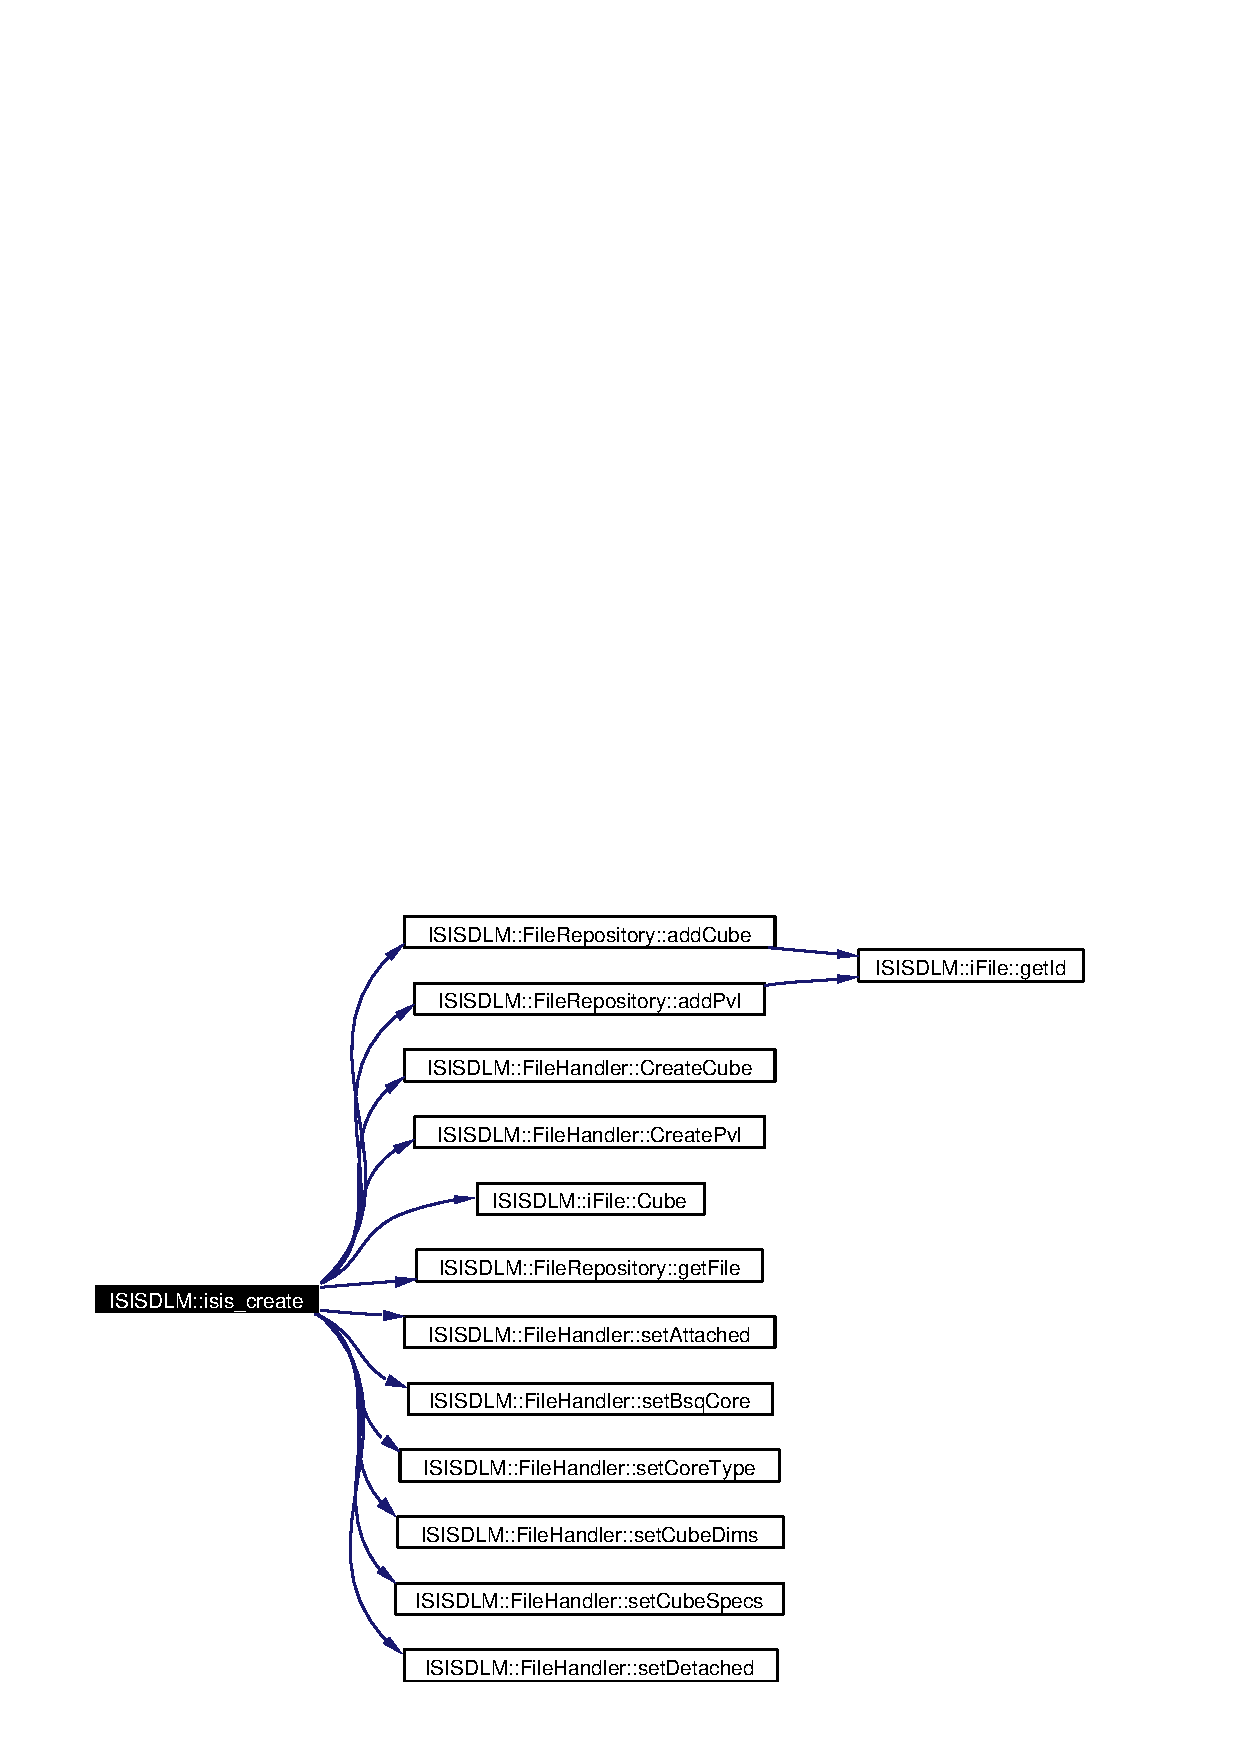
\includegraphics[width=264pt]{namespaceISISDLM_a14_cgraph}
\end{center}
\end{figure}
\index{ISISDLM@{ISISDLM}!isis_create_init@{isis\_\-create\_\-init}}
\index{isis_create_init@{isis\_\-create\_\-init}!ISISDLM@{ISISDLM}}
\subsubsection{\setlength{\rightskip}{0pt plus 5cm}int isis\_\-create\_\-init (Idl\-Dlm \& {\em idl})}\label{namespaceISISDLM_a13}


Performs initialization of isis\_\-create routine The isis\_\-create\_\-init function defines the isis\_\-create routine and registers it to the {\bf IDL} DLM toolkit. \begin{Desc}
\item[Parameters:]
\begin{description}
\item[{\em idl}]{\bf IDL} DLM interface \end{description}
\end{Desc}
\begin{Desc}
\item[Returns:]0 if successful, 1 otherwise \end{Desc}


Here is the call graph for this function:\begin{figure}[H]
\begin{center}
\leavevmode
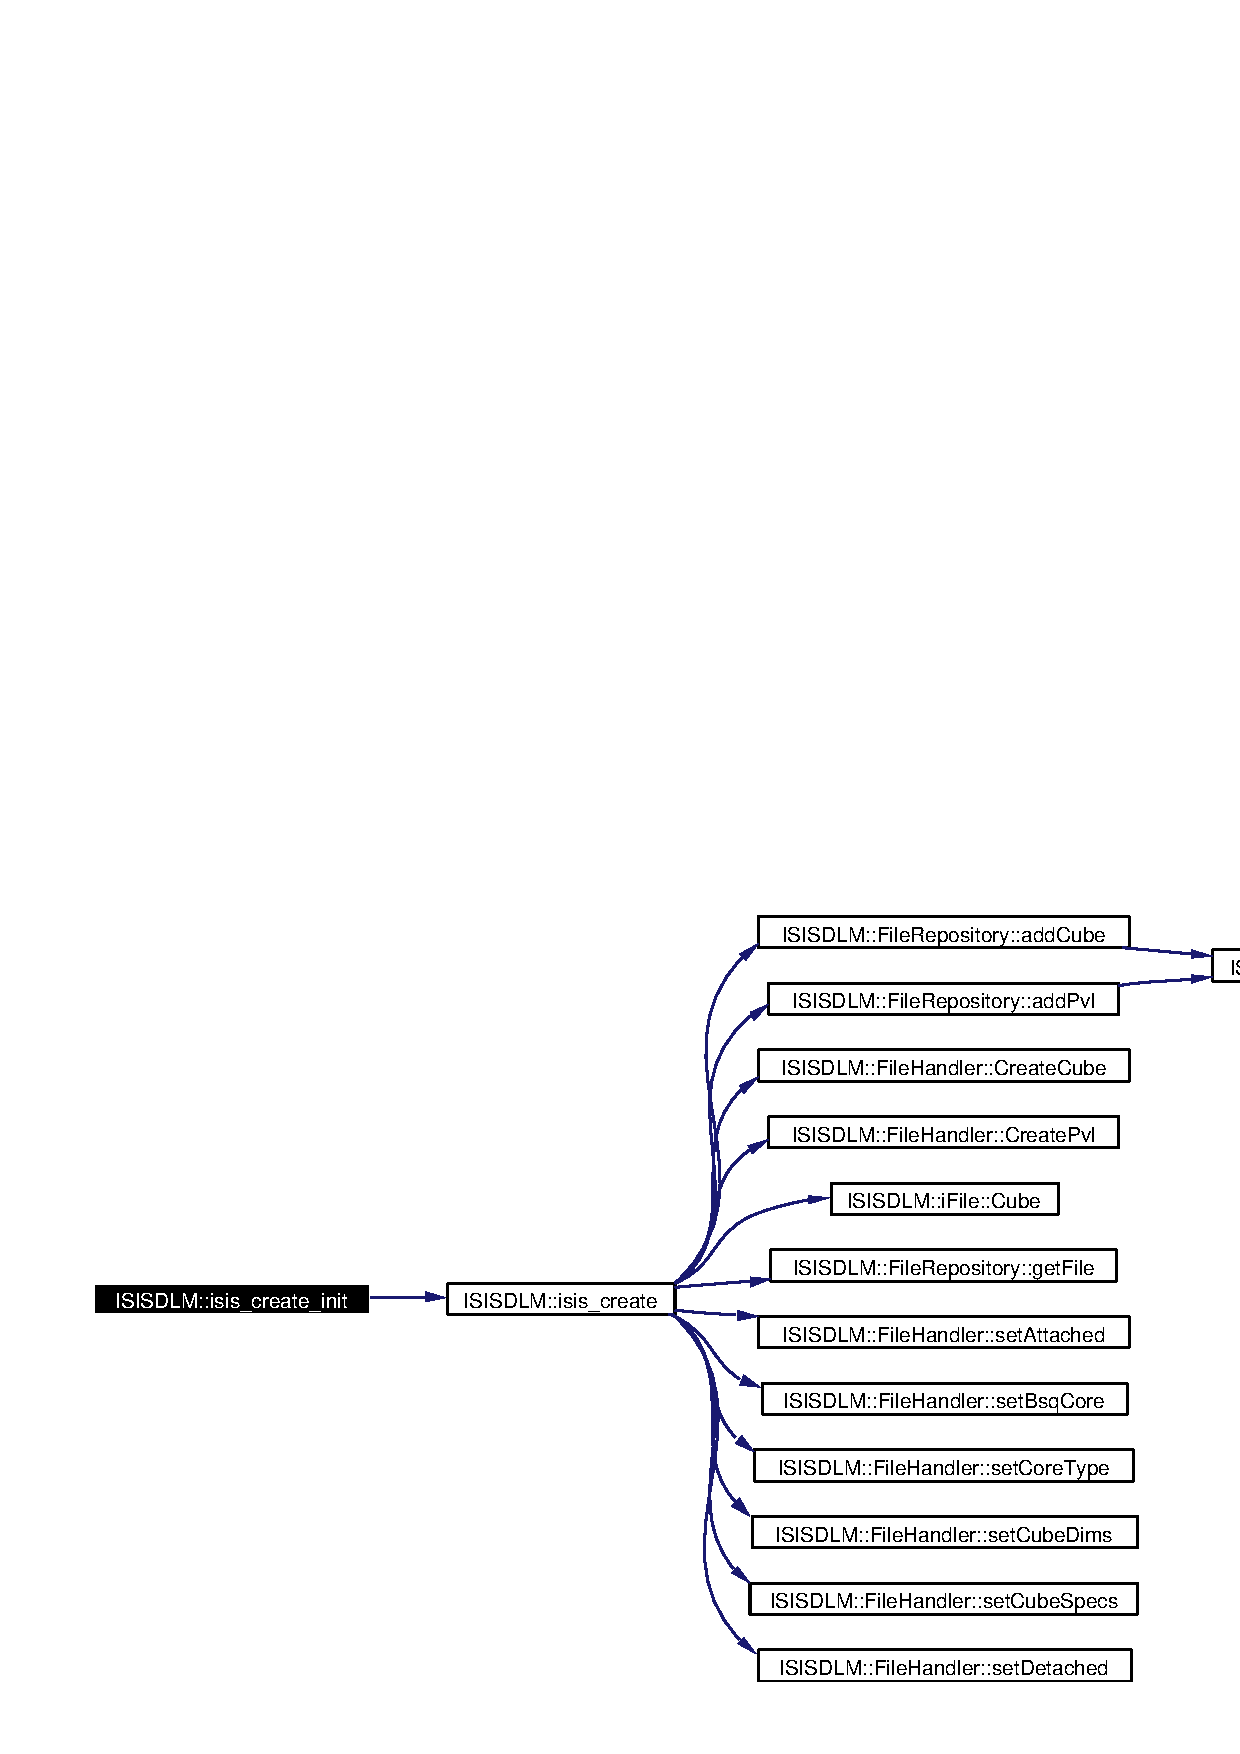
\includegraphics[width=349pt]{namespaceISISDLM_a13_cgraph}
\end{center}
\end{figure}
\index{ISISDLM@{ISISDLM}!isis_delete_aggregate@{isis\_\-delete\_\-aggregate}}
\index{isis_delete_aggregate@{isis\_\-delete\_\-aggregate}!ISISDLM@{ISISDLM}}
\subsubsection{\setlength{\rightskip}{0pt plus 5cm}int isis\_\-delete\_\-aggregate (const Idl\-Rtn\-Def \& {\em rtn}, const Idl\-Parameters \& {\em input}, Idl\-Parameters \& {\em output})}\label{namespaceISISDLM_a16}


Performs initialization of isis\_\-delete\_\-aggregate routine \begin{Desc}
\item[Parameters:]
\begin{description}
\item[{\em rtn}]Provides the function definition as specified in isis\_\-delete\_\-aggregate\_\-init \item[{\em input}]Contains a list of the input parameters \item[{\em output}]Will receive the parameters being passed back to {\bf IDL} user \end{description}
\end{Desc}
\begin{Desc}
\item[Returns:]0 if successful, 1 otherwise \end{Desc}
\index{ISISDLM@{ISISDLM}!isis_delete_aggregate_init@{isis\_\-delete\_\-aggregate\_\-init}}
\index{isis_delete_aggregate_init@{isis\_\-delete\_\-aggregate\_\-init}!ISISDLM@{ISISDLM}}
\subsubsection{\setlength{\rightskip}{0pt plus 5cm}int isis\_\-delete\_\-aggregate\_\-init (Idl\-Dlm \& {\em idl})}\label{namespaceISISDLM_a15}


Performs initialization of isis\_\-delete\_\-aggregate routine The isis\_\-delete\_\-aggregate\_\-init function defines the isis\_\-delete\_\-aggregate routine and registers it to the {\bf IDL} DLM toolkit. \begin{Desc}
\item[Parameters:]
\begin{description}
\item[{\em idl}]{\bf IDL} DLM interface \end{description}
\end{Desc}
\begin{Desc}
\item[Returns:]0 if successful, 1 otherwise \end{Desc}


Here is the call graph for this function:\begin{figure}[H]
\begin{center}
\leavevmode
\includegraphics[width=219pt]{namespaceISISDLM_a15_cgraph}
\end{center}
\end{figure}
\index{ISISDLM@{ISISDLM}!isis_get_key@{isis\_\-get\_\-key}}
\index{isis_get_key@{isis\_\-get\_\-key}!ISISDLM@{ISISDLM}}
\subsubsection{\setlength{\rightskip}{0pt plus 5cm}int isis\_\-get\_\-key (const Idl\-Rtn\-Def \& {\em rtn}, const Idl\-Parameters \& {\em input}, Idl\-Parameters \& {\em output})}\label{namespaceISISDLM_a18}


Performs initialization of isis\_\-get\_\-key routine \begin{Desc}
\item[Parameters:]
\begin{description}
\item[{\em rtn}]Provides the function definition as specified in isis\_\-get\_\-key\_\-init \item[{\em input}]Contains a list of the input parameters \item[{\em output}]Will receive the parameters being passed back to {\bf IDL} user \end{description}
\end{Desc}
\begin{Desc}
\item[Returns:]0 if successful, 1 otherwise \end{Desc}


Here is the call graph for this function:\begin{figure}[H]
\begin{center}
\leavevmode
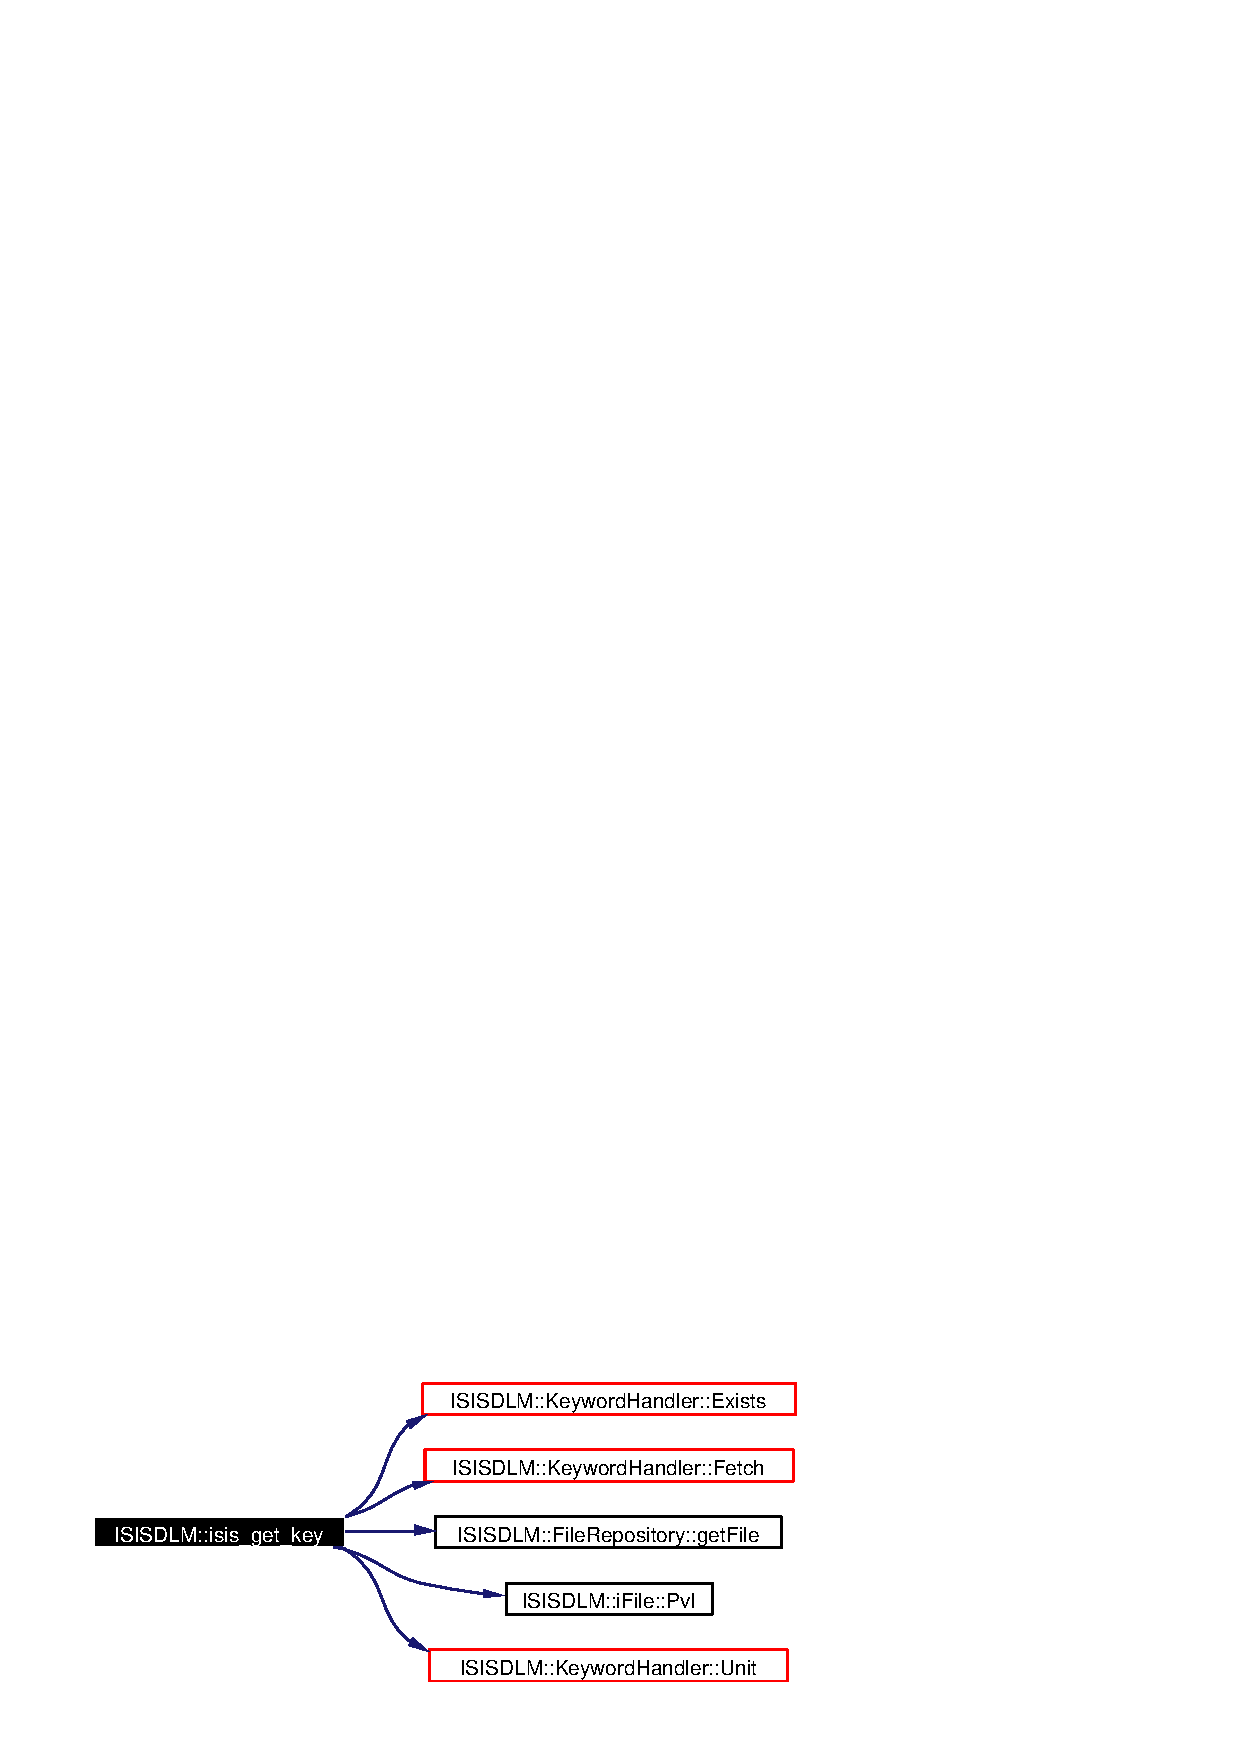
\includegraphics[width=195pt]{namespaceISISDLM_a18_cgraph}
\end{center}
\end{figure}
\index{ISISDLM@{ISISDLM}!isis_get_key_init@{isis\_\-get\_\-key\_\-init}}
\index{isis_get_key_init@{isis\_\-get\_\-key\_\-init}!ISISDLM@{ISISDLM}}
\subsubsection{\setlength{\rightskip}{0pt plus 5cm}int isis\_\-get\_\-key\_\-init (Idl\-Dlm \& {\em idl})}\label{namespaceISISDLM_a17}


Performs initialization of isis\_\-query routine The isis\_\-get\_\-key\_\-init function defines the isis\_\-get\_\-key routine and registers it to the {\bf IDL} DLM toolkit. \begin{Desc}
\item[Parameters:]
\begin{description}
\item[{\em idl}]{\bf IDL} DLM interface \end{description}
\end{Desc}
\begin{Desc}
\item[Returns:]0 if successful, 1 otherwise \end{Desc}


Here is the call graph for this function:\begin{figure}[H]
\begin{center}
\leavevmode
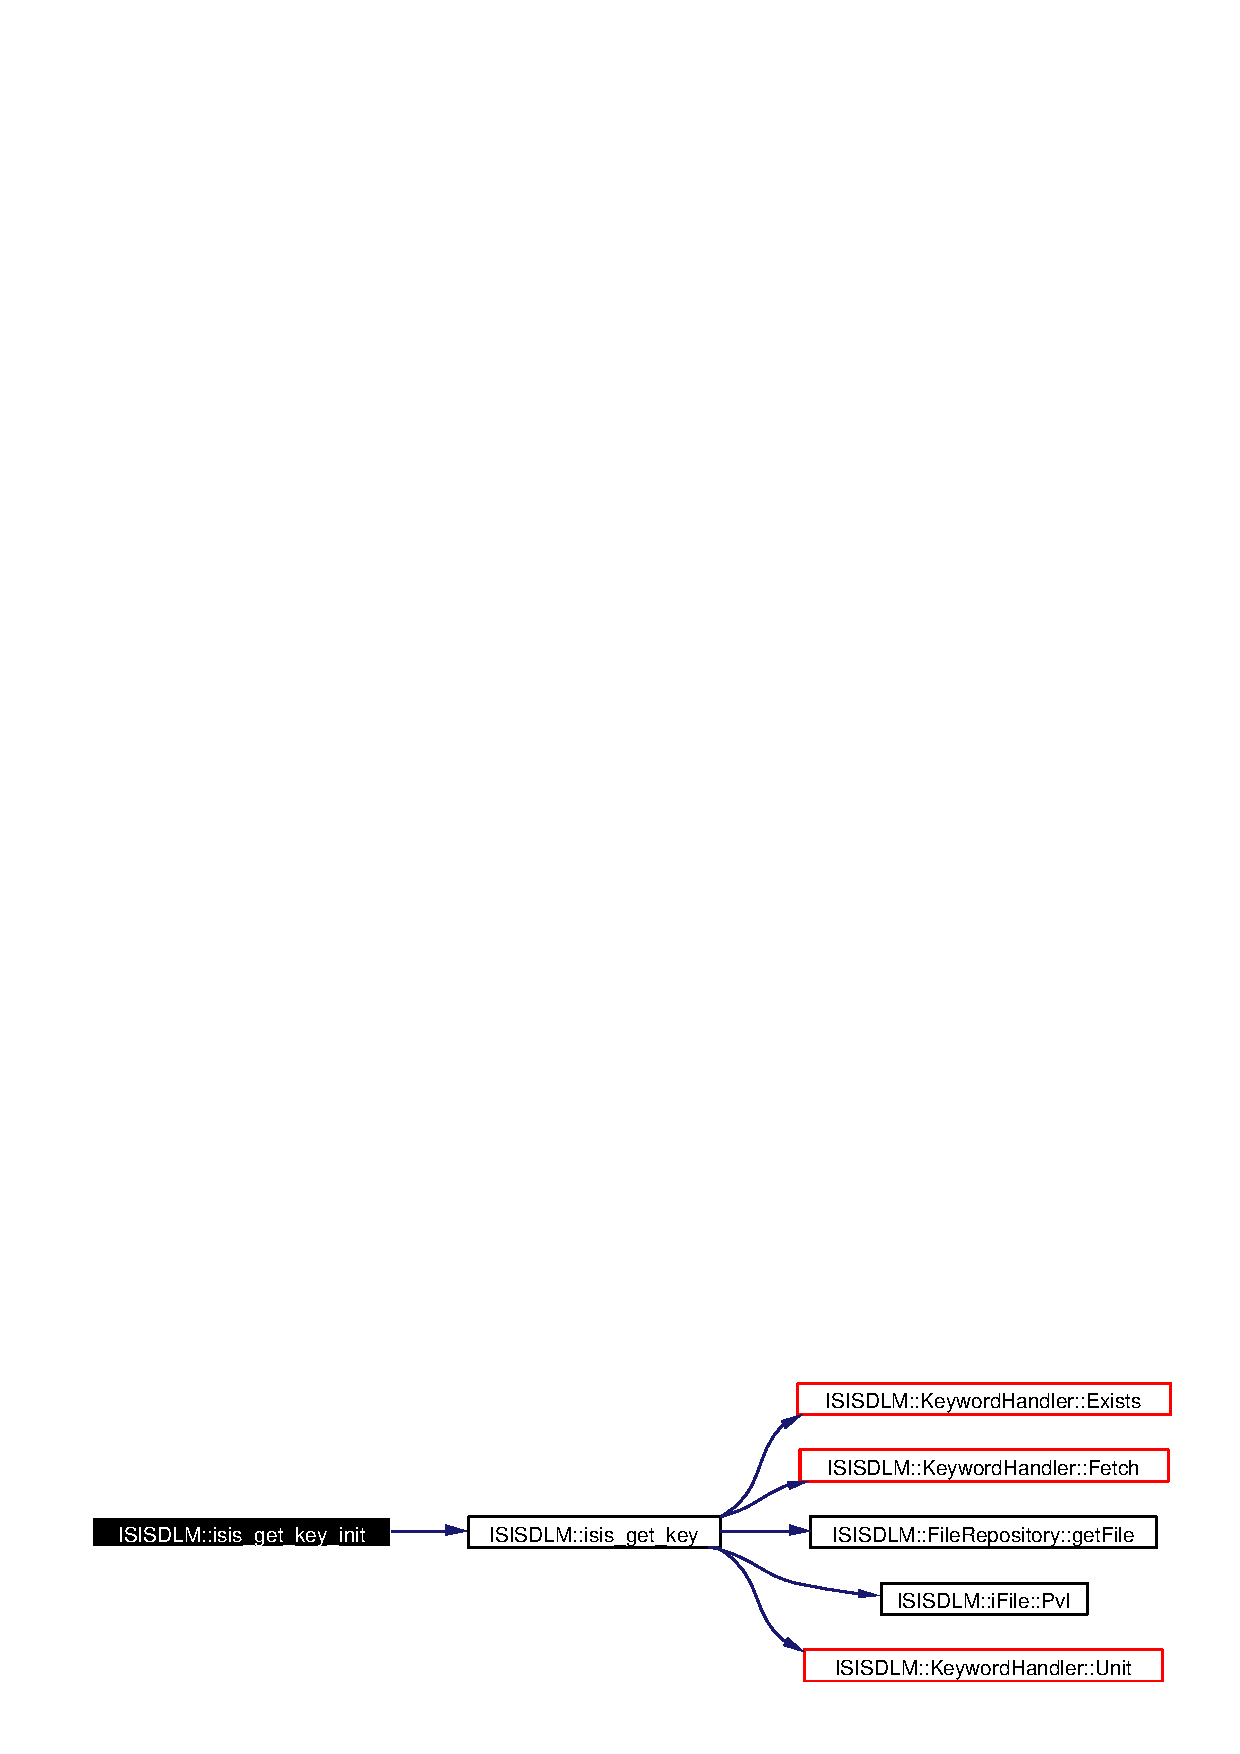
\includegraphics[width=285pt]{namespaceISISDLM_a17_cgraph}
\end{center}
\end{figure}
\index{ISISDLM@{ISISDLM}!isis_open@{isis\_\-open}}
\index{isis_open@{isis\_\-open}!ISISDLM@{ISISDLM}}
\subsubsection{\setlength{\rightskip}{0pt plus 5cm}int isis\_\-open (const Idl\-Rtn\-Def \& {\em rtn}, const Idl\-Parameters \& {\em input}, Idl\-Parameters \& {\em output})}\label{namespaceISISDLM_a20}


Performs initialization of isis\_\-open routine \begin{Desc}
\item[Parameters:]
\begin{description}
\item[{\em rtn}]Provides the function definition as specified in isis\_\-open\_\-init \item[{\em input}]Contains a list of the input parameters \item[{\em output}]Will receive the parameters being passed back to {\bf IDL} user \end{description}
\end{Desc}
\begin{Desc}
\item[Returns:]0 if successful, 1 otherwise \end{Desc}


Here is the call graph for this function:\begin{figure}[H]
\begin{center}
\leavevmode
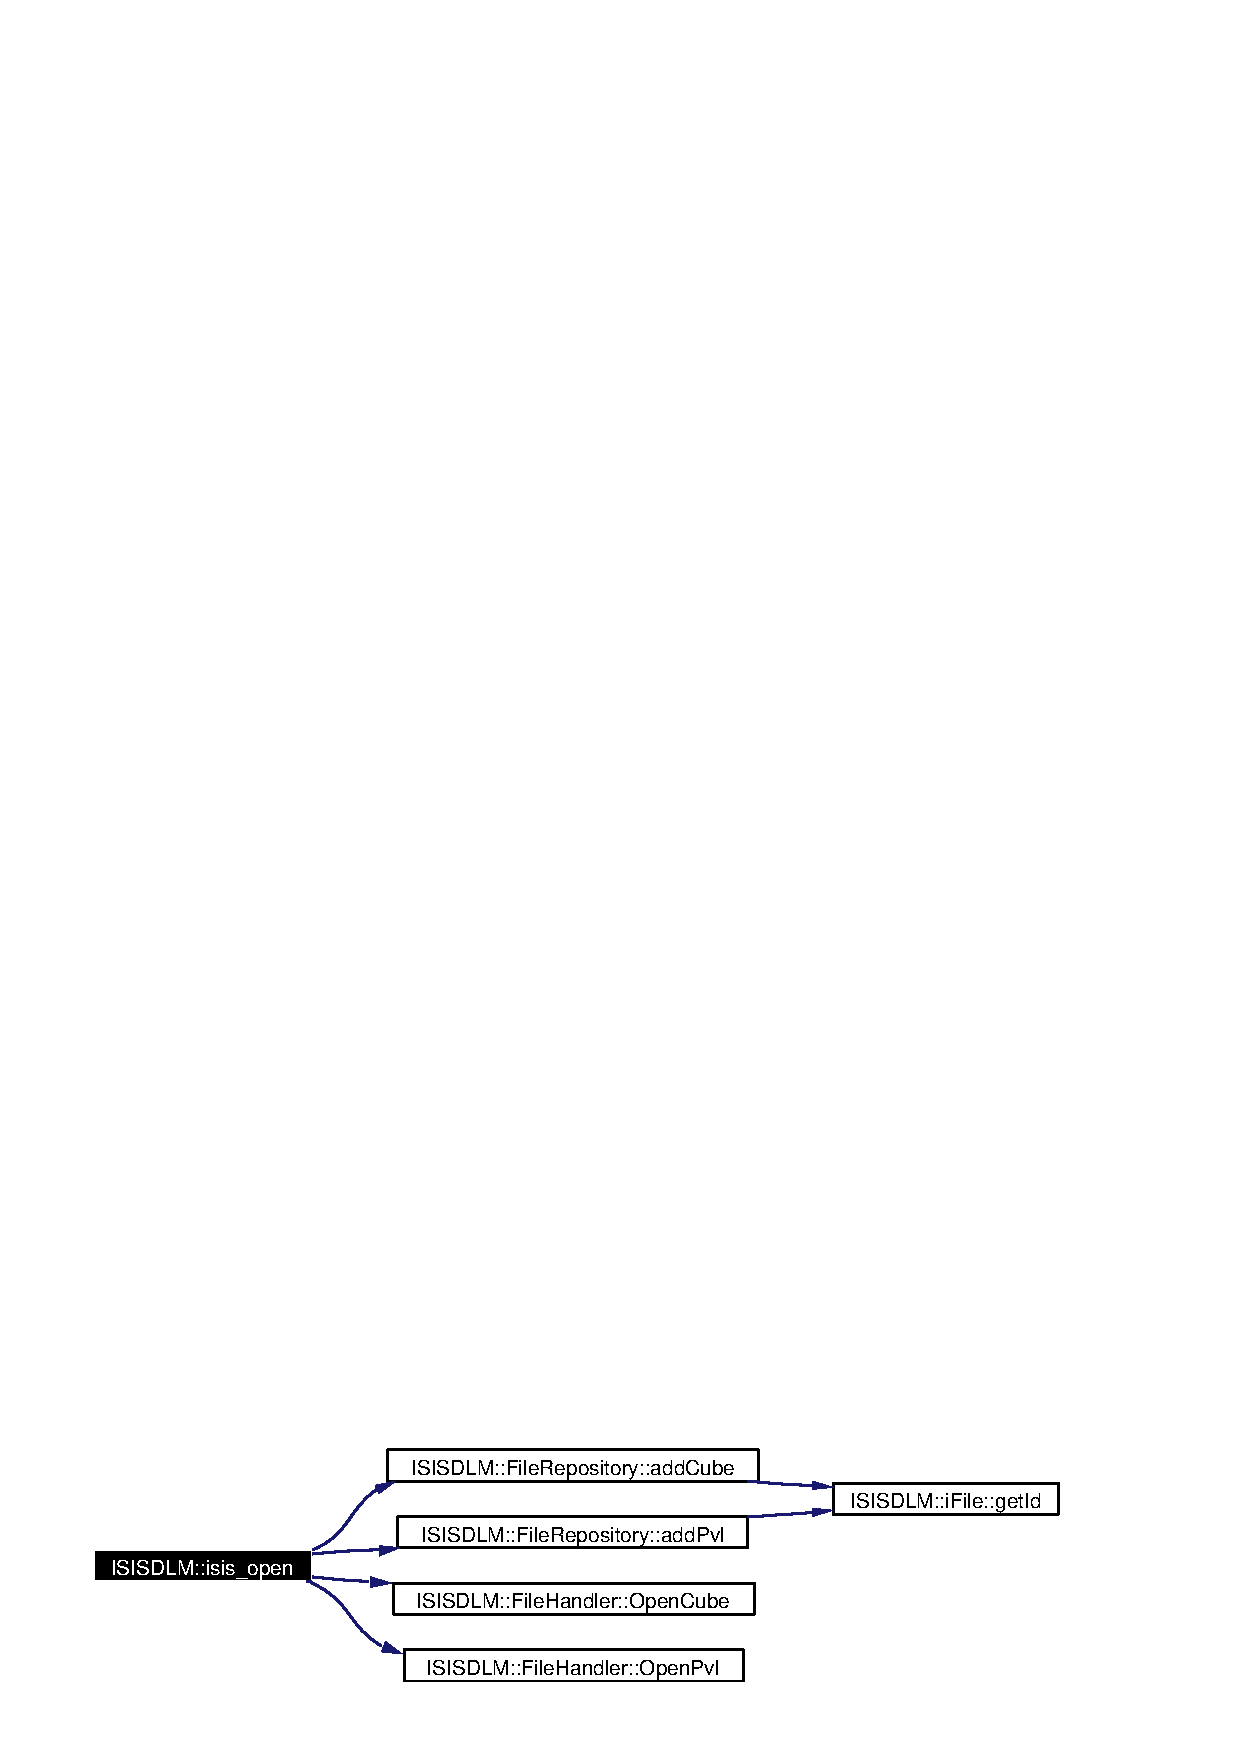
\includegraphics[width=258pt]{namespaceISISDLM_a20_cgraph}
\end{center}
\end{figure}
\index{ISISDLM@{ISISDLM}!isis_open_init@{isis\_\-open\_\-init}}
\index{isis_open_init@{isis\_\-open\_\-init}!ISISDLM@{ISISDLM}}
\subsubsection{\setlength{\rightskip}{0pt plus 5cm}int isis\_\-open\_\-init (Idl\-Dlm \& {\em idl})}\label{namespaceISISDLM_a19}


Performs initialization of isis\_\-open routine The isis\_\-open\_\-init function defines the isis\_\-open routine and registers it to the {\bf IDL} DLM toolkit. \begin{Desc}
\item[Parameters:]
\begin{description}
\item[{\em idl}]{\bf IDL} DLM interface \end{description}
\end{Desc}
\begin{Desc}
\item[Returns:]0 if successful, 1 otherwise \end{Desc}


Here is the call graph for this function:\begin{figure}[H]
\begin{center}
\leavevmode
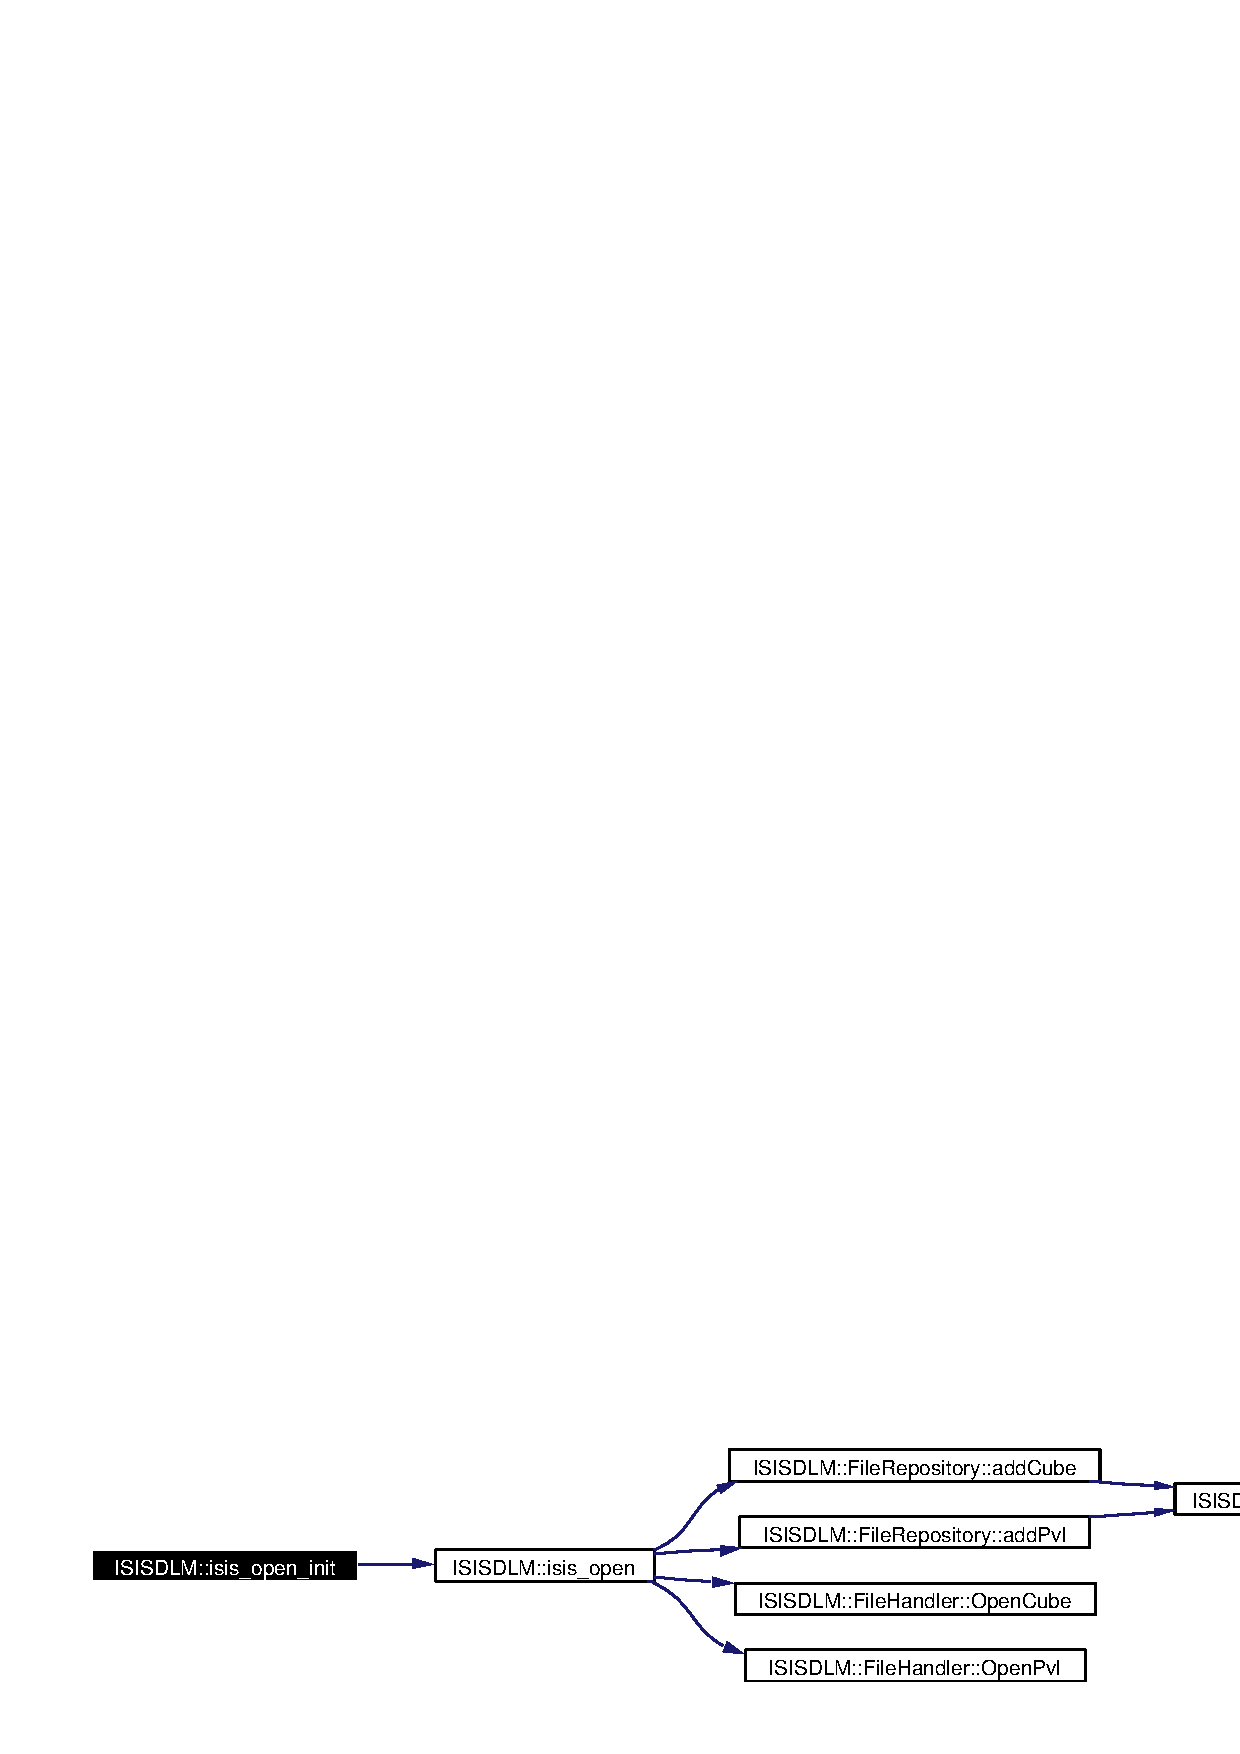
\includegraphics[width=340pt]{namespaceISISDLM_a19_cgraph}
\end{center}
\end{figure}
\index{ISISDLM@{ISISDLM}!isis_query@{isis\_\-query}}
\index{isis_query@{isis\_\-query}!ISISDLM@{ISISDLM}}
\subsubsection{\setlength{\rightskip}{0pt plus 5cm}int isis\_\-query (const Idl\-Rtn\-Def \& {\em rtn}, const Idl\-Parameters \& {\em input}, Idl\-Parameters \& {\em output})}\label{namespaceISISDLM_a23}


Performs initialization of isis\_\-query routine \begin{Desc}
\item[Parameters:]
\begin{description}
\item[{\em rtn}]Provides the function definition as specified in isis\_\-query\_\-init \item[{\em input}]Contains a list of the input parameters \item[{\em output}]Will receive the parameters being passed back to {\bf IDL} user \end{description}
\end{Desc}
\begin{Desc}
\item[Returns:]0 if successful, 1 otherwise \end{Desc}


Here is the call graph for this function:\begin{figure}[H]
\begin{center}
\leavevmode
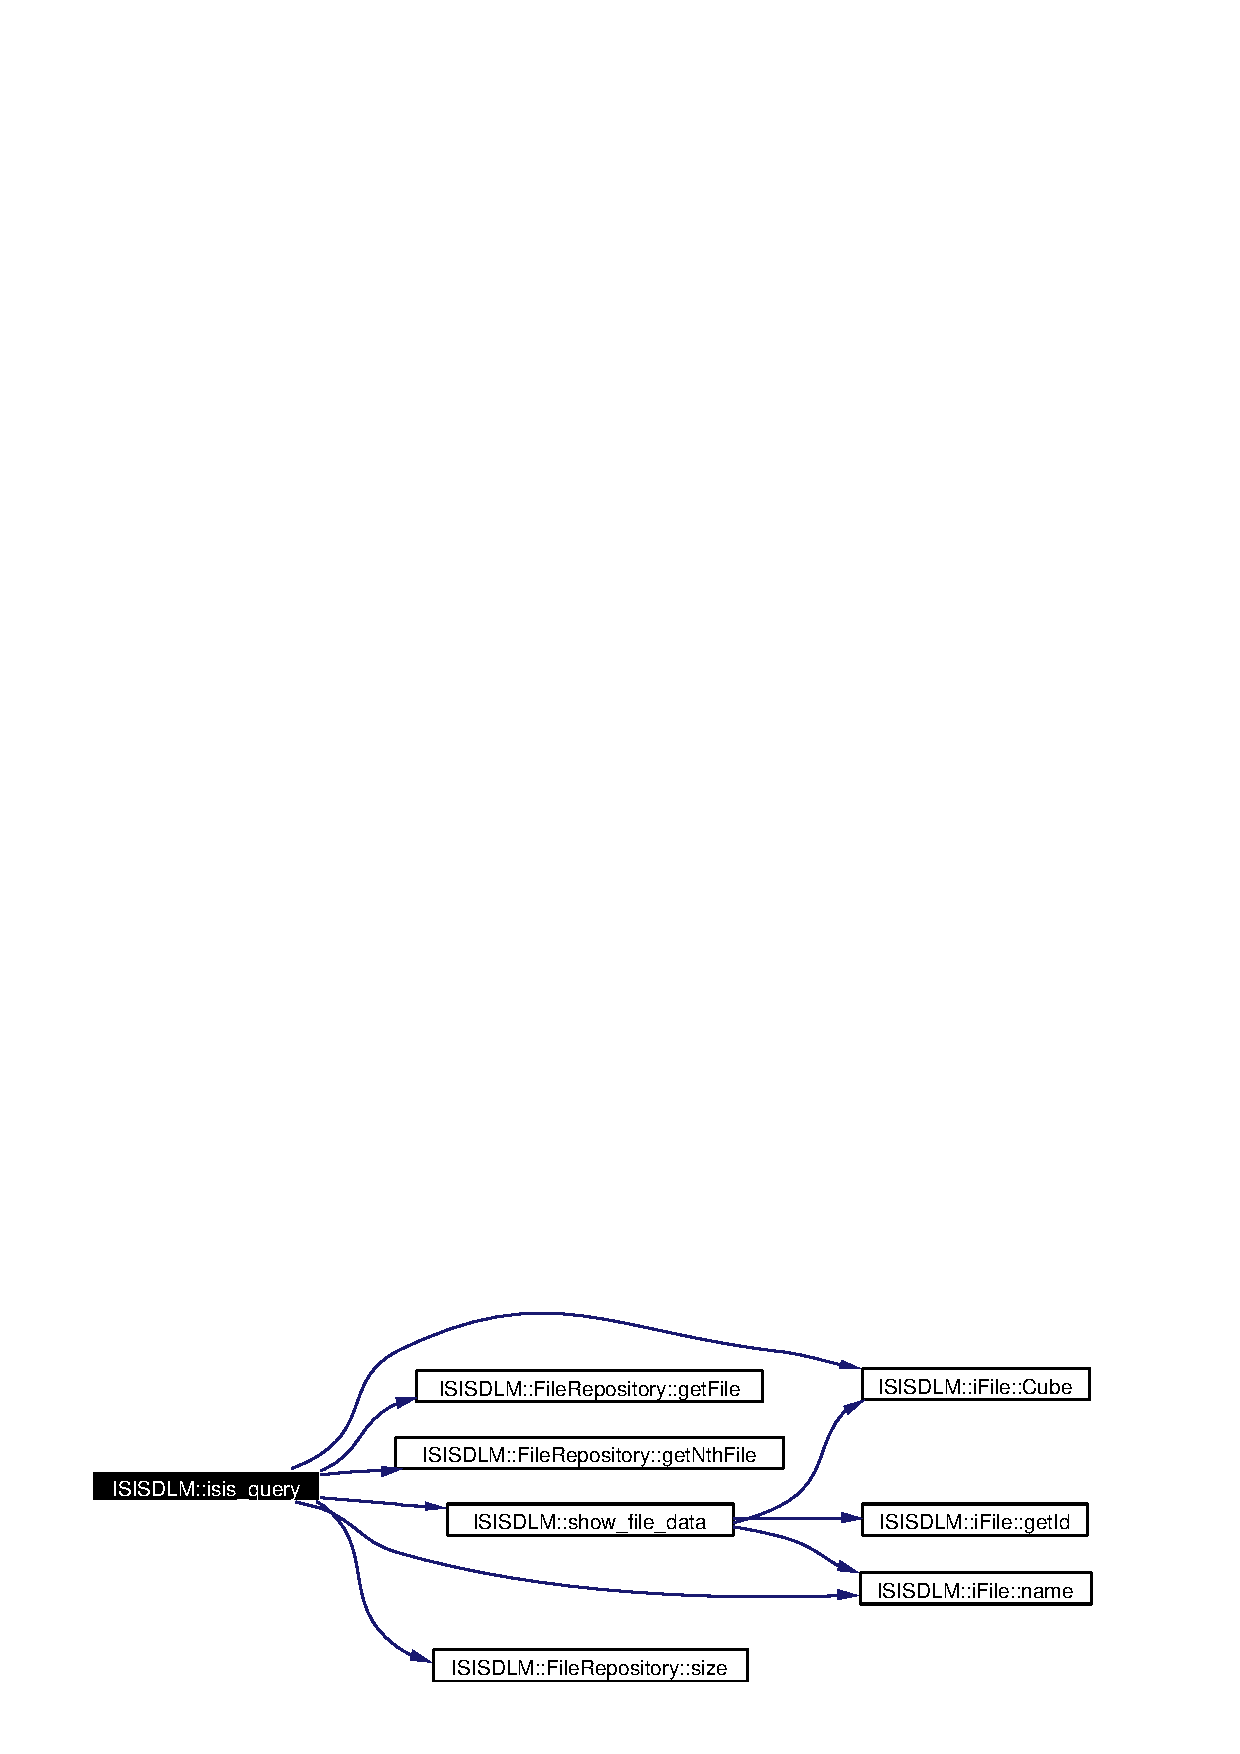
\includegraphics[width=266pt]{namespaceISISDLM_a23_cgraph}
\end{center}
\end{figure}
\index{ISISDLM@{ISISDLM}!isis_query_init@{isis\_\-query\_\-init}}
\index{isis_query_init@{isis\_\-query\_\-init}!ISISDLM@{ISISDLM}}
\subsubsection{\setlength{\rightskip}{0pt plus 5cm}int isis\_\-query\_\-init (Idl\-Dlm \& {\em idl})}\label{namespaceISISDLM_a21}


Performs initialization of isis\_\-query routine The isis\_\-query\_\-init function defines the isis\_\-query routine and registers it to the {\bf IDL} DLM toolkit. \begin{Desc}
\item[Parameters:]
\begin{description}
\item[{\em idl}]{\bf IDL} DLM interface \end{description}
\end{Desc}
\begin{Desc}
\item[Returns:]0 if successful, 1 otherwise \end{Desc}


Here is the call graph for this function:\begin{figure}[H]
\begin{center}
\leavevmode
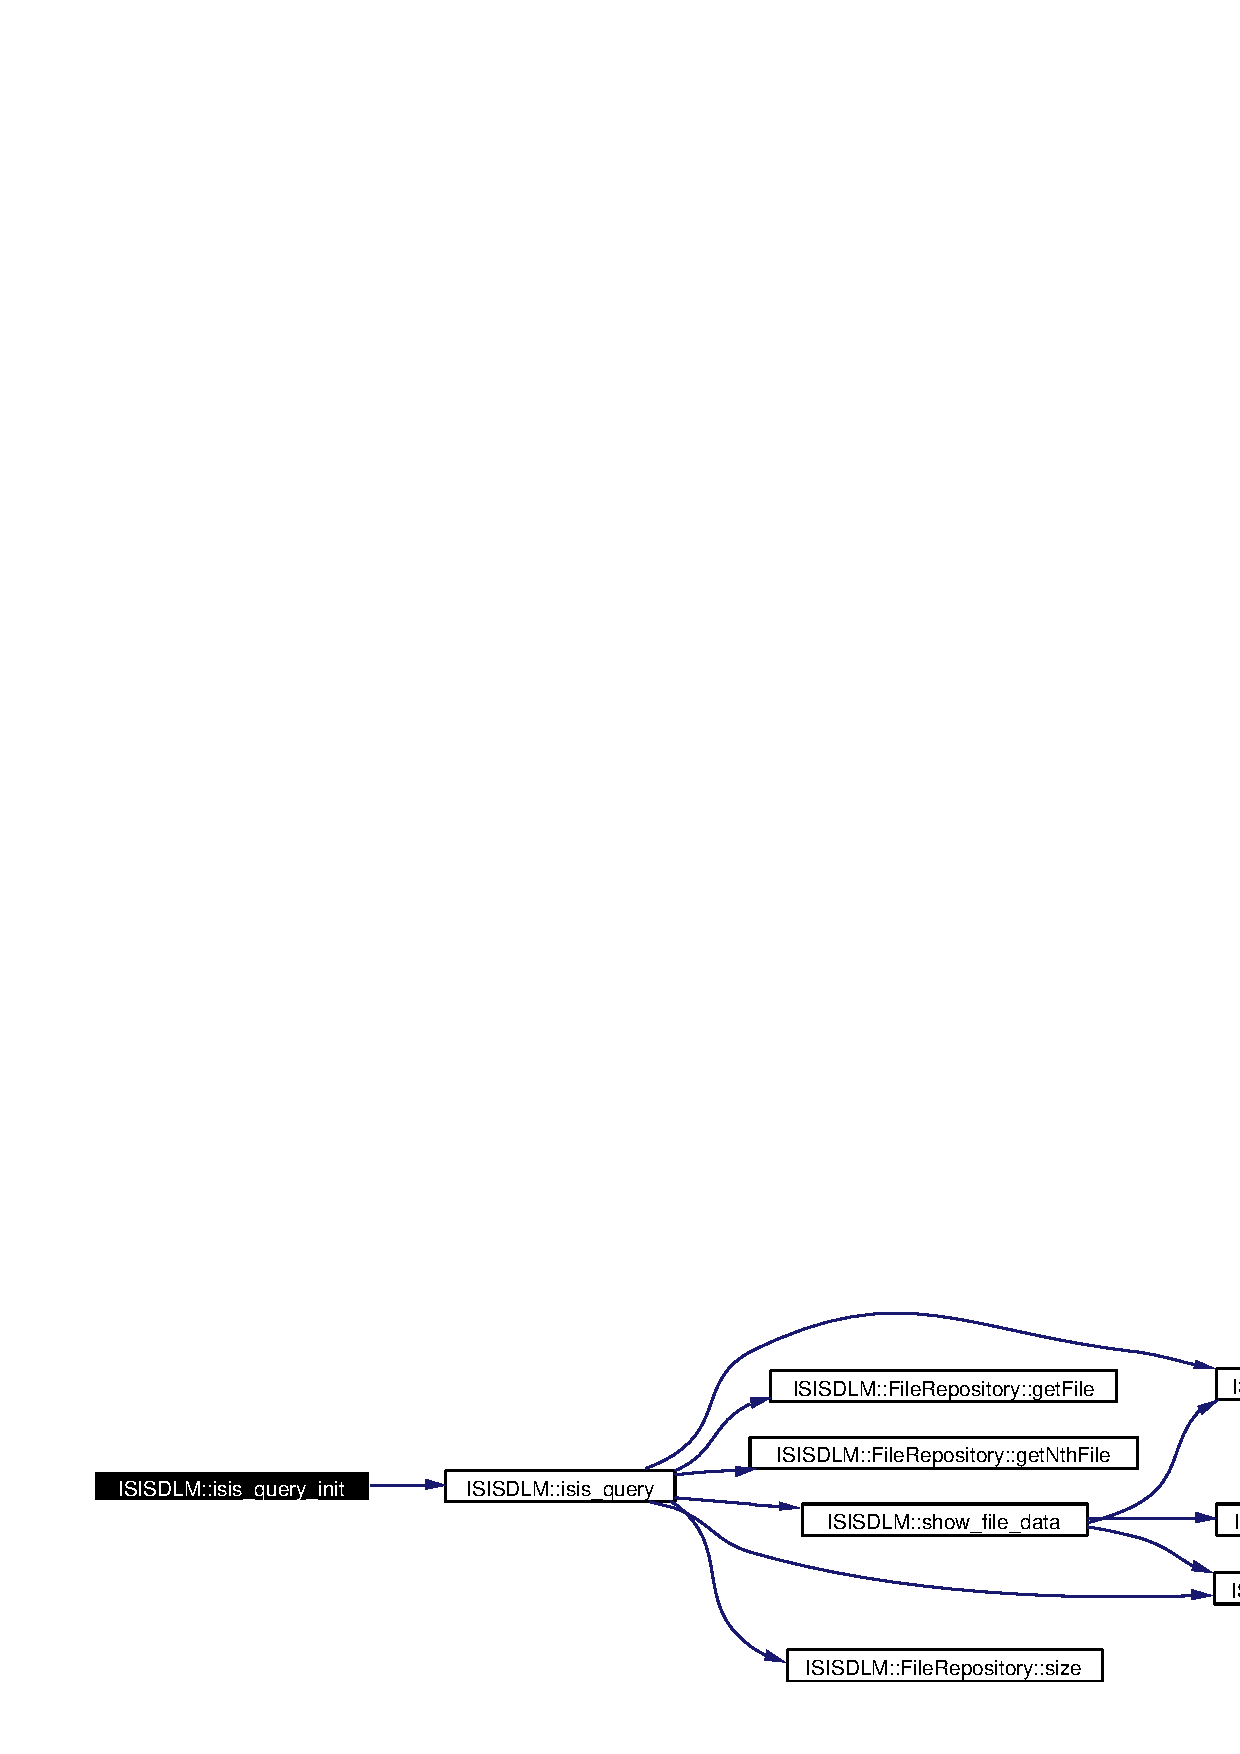
\includegraphics[width=351pt]{namespaceISISDLM_a21_cgraph}
\end{center}
\end{figure}
\index{ISISDLM@{ISISDLM}!isis_query_key@{isis\_\-query\_\-key}}
\index{isis_query_key@{isis\_\-query\_\-key}!ISISDLM@{ISISDLM}}
\subsubsection{\setlength{\rightskip}{0pt plus 5cm}int isis\_\-query\_\-key (const Idl\-Rtn\-Def \& {\em rtn}, const Idl\-Parameters \& {\em input}, Idl\-Parameters \& {\em output})}\label{namespaceISISDLM_a25}


Performs initialization of isis\_\-query\_\-key routine \begin{Desc}
\item[Parameters:]
\begin{description}
\item[{\em rtn}]Provides the function definition as specified in isis\_\-query\_\-key\_\-init \item[{\em input}]Contains a list of the input parameters \item[{\em output}]Will receive the parameters being passed back to {\bf IDL} user \end{description}
\end{Desc}
\begin{Desc}
\item[Returns:]0 if successful, 1 otherwise \end{Desc}


Here is the call graph for this function:\begin{figure}[H]
\begin{center}
\leavevmode
\includegraphics[width=202pt]{namespaceISISDLM_a25_cgraph}
\end{center}
\end{figure}
\index{ISISDLM@{ISISDLM}!isis_query_key_init@{isis\_\-query\_\-key\_\-init}}
\index{isis_query_key_init@{isis\_\-query\_\-key\_\-init}!ISISDLM@{ISISDLM}}
\subsubsection{\setlength{\rightskip}{0pt plus 5cm}int isis\_\-query\_\-key\_\-init (Idl\-Dlm \& {\em idl})}\label{namespaceISISDLM_a24}


Performs initialization of isis\_\-query routine The isis\_\-query\_\-key\_\-init function defines the isis\_\-query\_\-key routine and registers it to the {\bf IDL} DLM toolkit. \begin{Desc}
\item[Parameters:]
\begin{description}
\item[{\em idl}]{\bf IDL} DLM interface \end{description}
\end{Desc}
\begin{Desc}
\item[Returns:]0 if successful, 1 otherwise \end{Desc}


Here is the call graph for this function:\begin{figure}[H]
\begin{center}
\leavevmode
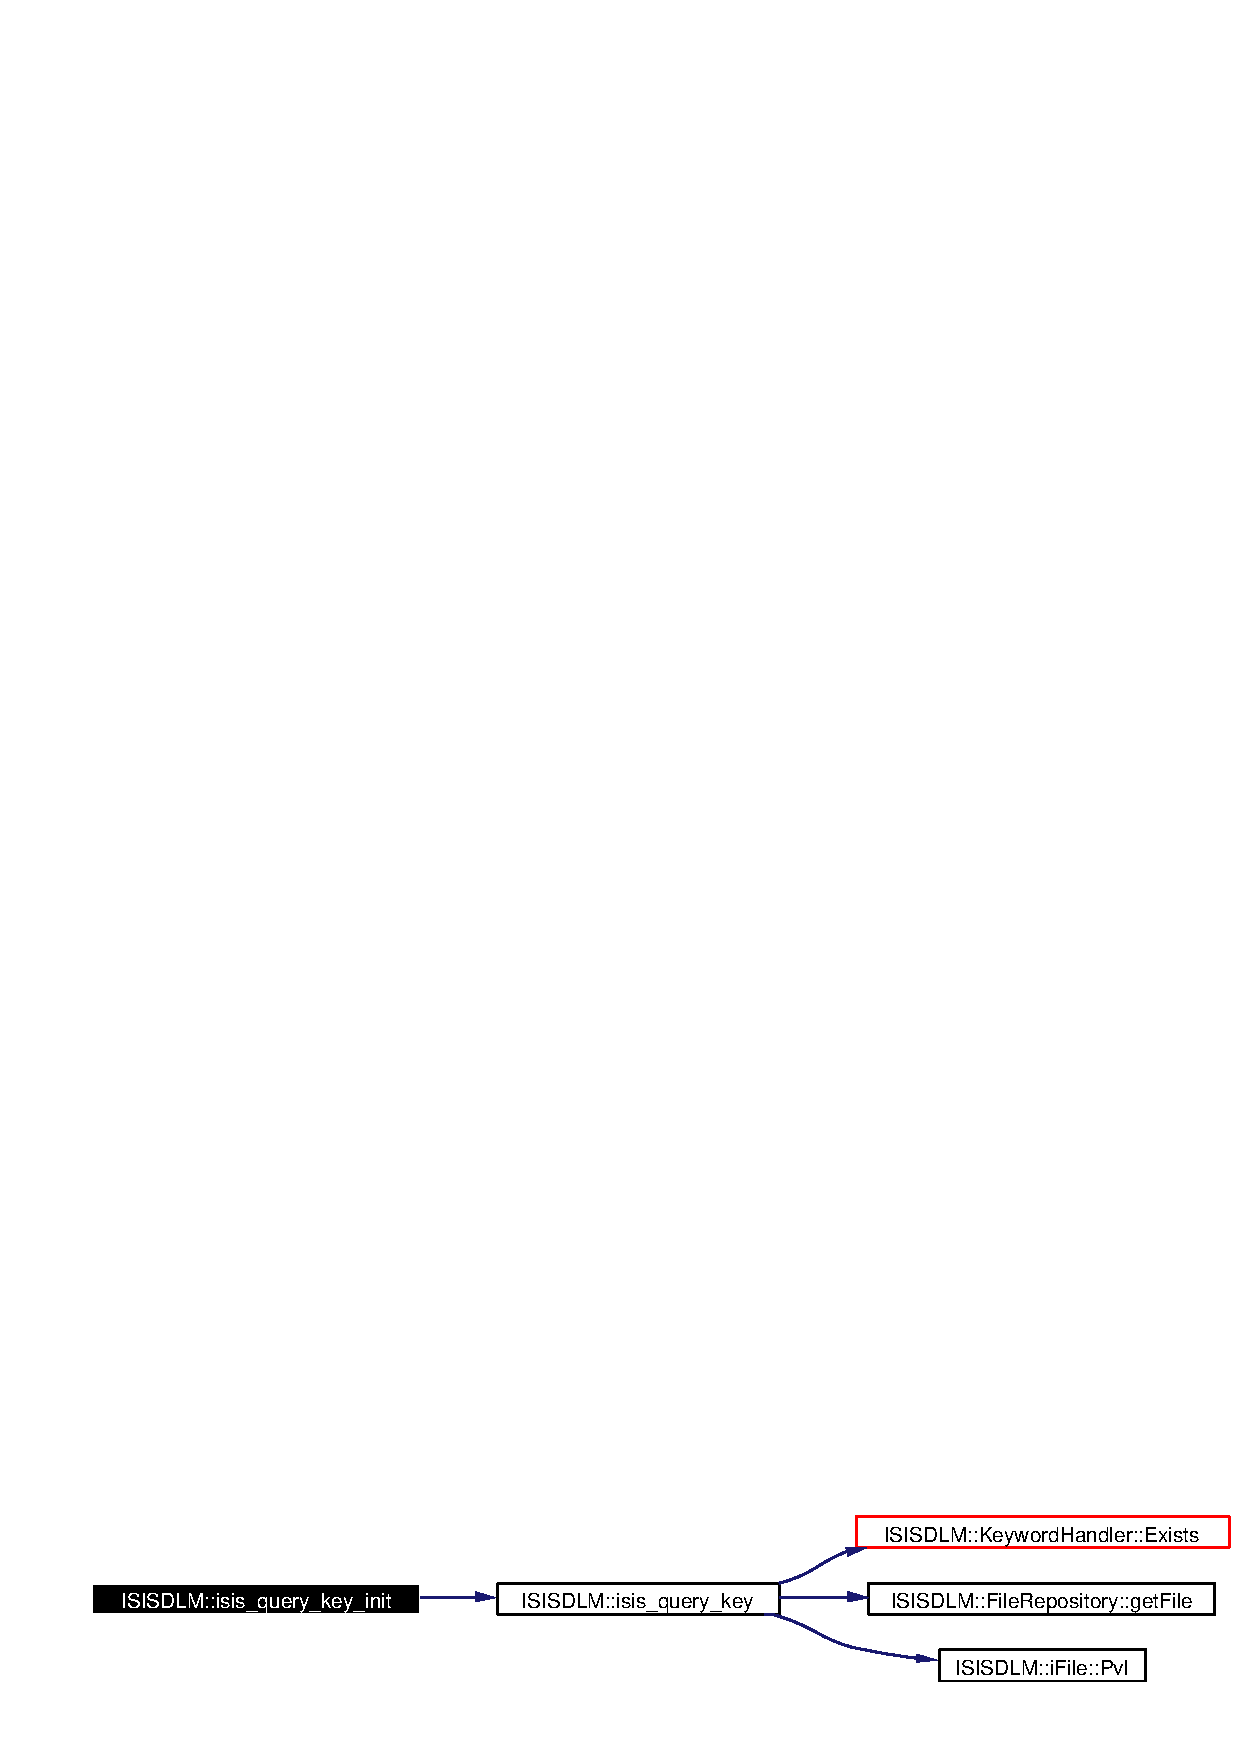
\includegraphics[width=299pt]{namespaceISISDLM_a24_cgraph}
\end{center}
\end{figure}
\index{ISISDLM@{ISISDLM}!isis_read@{isis\_\-read}}
\index{isis_read@{isis\_\-read}!ISISDLM@{ISISDLM}}
\subsubsection{\setlength{\rightskip}{0pt plus 5cm}int isis\_\-read (const Idl\-Rtn\-Def \& {\em rtn}, const Idl\-Parameters \& {\em input}, Idl\-Parameters \& {\em output})}\label{namespaceISISDLM_a27}


Performs initialization of isis\_\-read routine \begin{Desc}
\item[Parameters:]
\begin{description}
\item[{\em rtn}]Provides the function definition as specified in isis\_\-read\_\-init \item[{\em input}]Contains a list of the input parameters \item[{\em output}]Will receive the parameters being passed back to {\bf IDL} user \end{description}
\end{Desc}
\begin{Desc}
\item[Returns:]0 if successful, 1 otherwise \end{Desc}


Here is the call graph for this function:\begin{figure}[H]
\begin{center}
\leavevmode
\includegraphics[width=256pt]{namespaceISISDLM_a27_cgraph}
\end{center}
\end{figure}
\index{ISISDLM@{ISISDLM}!isis_read_blob@{isis\_\-read\_\-blob}}
\index{isis_read_blob@{isis\_\-read\_\-blob}!ISISDLM@{ISISDLM}}
\subsubsection{\setlength{\rightskip}{0pt plus 5cm}int isis\_\-read\_\-blob (const Idl\-Rtn\-Def \& {\em rtn}, const Idl\-Parameters \& {\em input}, Idl\-Parameters \& {\em output})}\label{namespaceISISDLM_a29}


Performs initialization of isis\_\-read\_\-blob routine \begin{Desc}
\item[Parameters:]
\begin{description}
\item[{\em rtn}]Provides the function definition as specified in isis\_\-read\_\-blob\_\-init \item[{\em input}]Contains a list of the input parameters \item[{\em output}]Will receive the parameters being passed back to {\bf IDL} user \end{description}
\end{Desc}
\begin{Desc}
\item[Returns:]0 if successful, 1 otherwise \end{Desc}


Here is the call graph for this function:\begin{figure}[H]
\begin{center}
\leavevmode
\includegraphics[width=193pt]{namespaceISISDLM_a29_cgraph}
\end{center}
\end{figure}
\index{ISISDLM@{ISISDLM}!isis_read_blob_init@{isis\_\-read\_\-blob\_\-init}}
\index{isis_read_blob_init@{isis\_\-read\_\-blob\_\-init}!ISISDLM@{ISISDLM}}
\subsubsection{\setlength{\rightskip}{0pt plus 5cm}int isis\_\-read\_\-blob\_\-init (Idl\-Dlm \& {\em idl})}\label{namespaceISISDLM_a28}


Performs initialization of isis\_\-read\_\-blob routine The isis\_\-read\_\-blob\_\-init function defines the isis\_\-read\_\-blob routine and registers it to the {\bf IDL} DLM toolkit. \begin{Desc}
\item[Parameters:]
\begin{description}
\item[{\em idl}]{\bf IDL} DLM interface \end{description}
\end{Desc}
\begin{Desc}
\item[Returns:]0 if successful, 1 otherwise \end{Desc}


Here is the call graph for this function:\begin{figure}[H]
\begin{center}
\leavevmode
\includegraphics[width=288pt]{namespaceISISDLM_a28_cgraph}
\end{center}
\end{figure}
\index{ISISDLM@{ISISDLM}!isis_read_brick@{isis\_\-read\_\-brick}}
\index{isis_read_brick@{isis\_\-read\_\-brick}!ISISDLM@{ISISDLM}}
\subsubsection{\setlength{\rightskip}{0pt plus 5cm}int isis\_\-read\_\-brick (const Idl\-Rtn\-Def \& {\em rtn}, const Idl\-Parameters \& {\em input}, Idl\-Parameters \& {\em output})}\label{namespaceISISDLM_a31}


Performs initialization of isis\_\-read\_\-brick routine \begin{Desc}
\item[Parameters:]
\begin{description}
\item[{\em rtn}]Provides the function definition as specified in isis\_\-read\_\-brick\_\-init \item[{\em input}]Contains a list of the input parameters \item[{\em output}]Will receive the parameters being passed back to {\bf IDL} user \end{description}
\end{Desc}
\begin{Desc}
\item[Returns:]0 if successful, 1 otherwise \end{Desc}


Here is the call graph for this function:\begin{figure}[H]
\begin{center}
\leavevmode
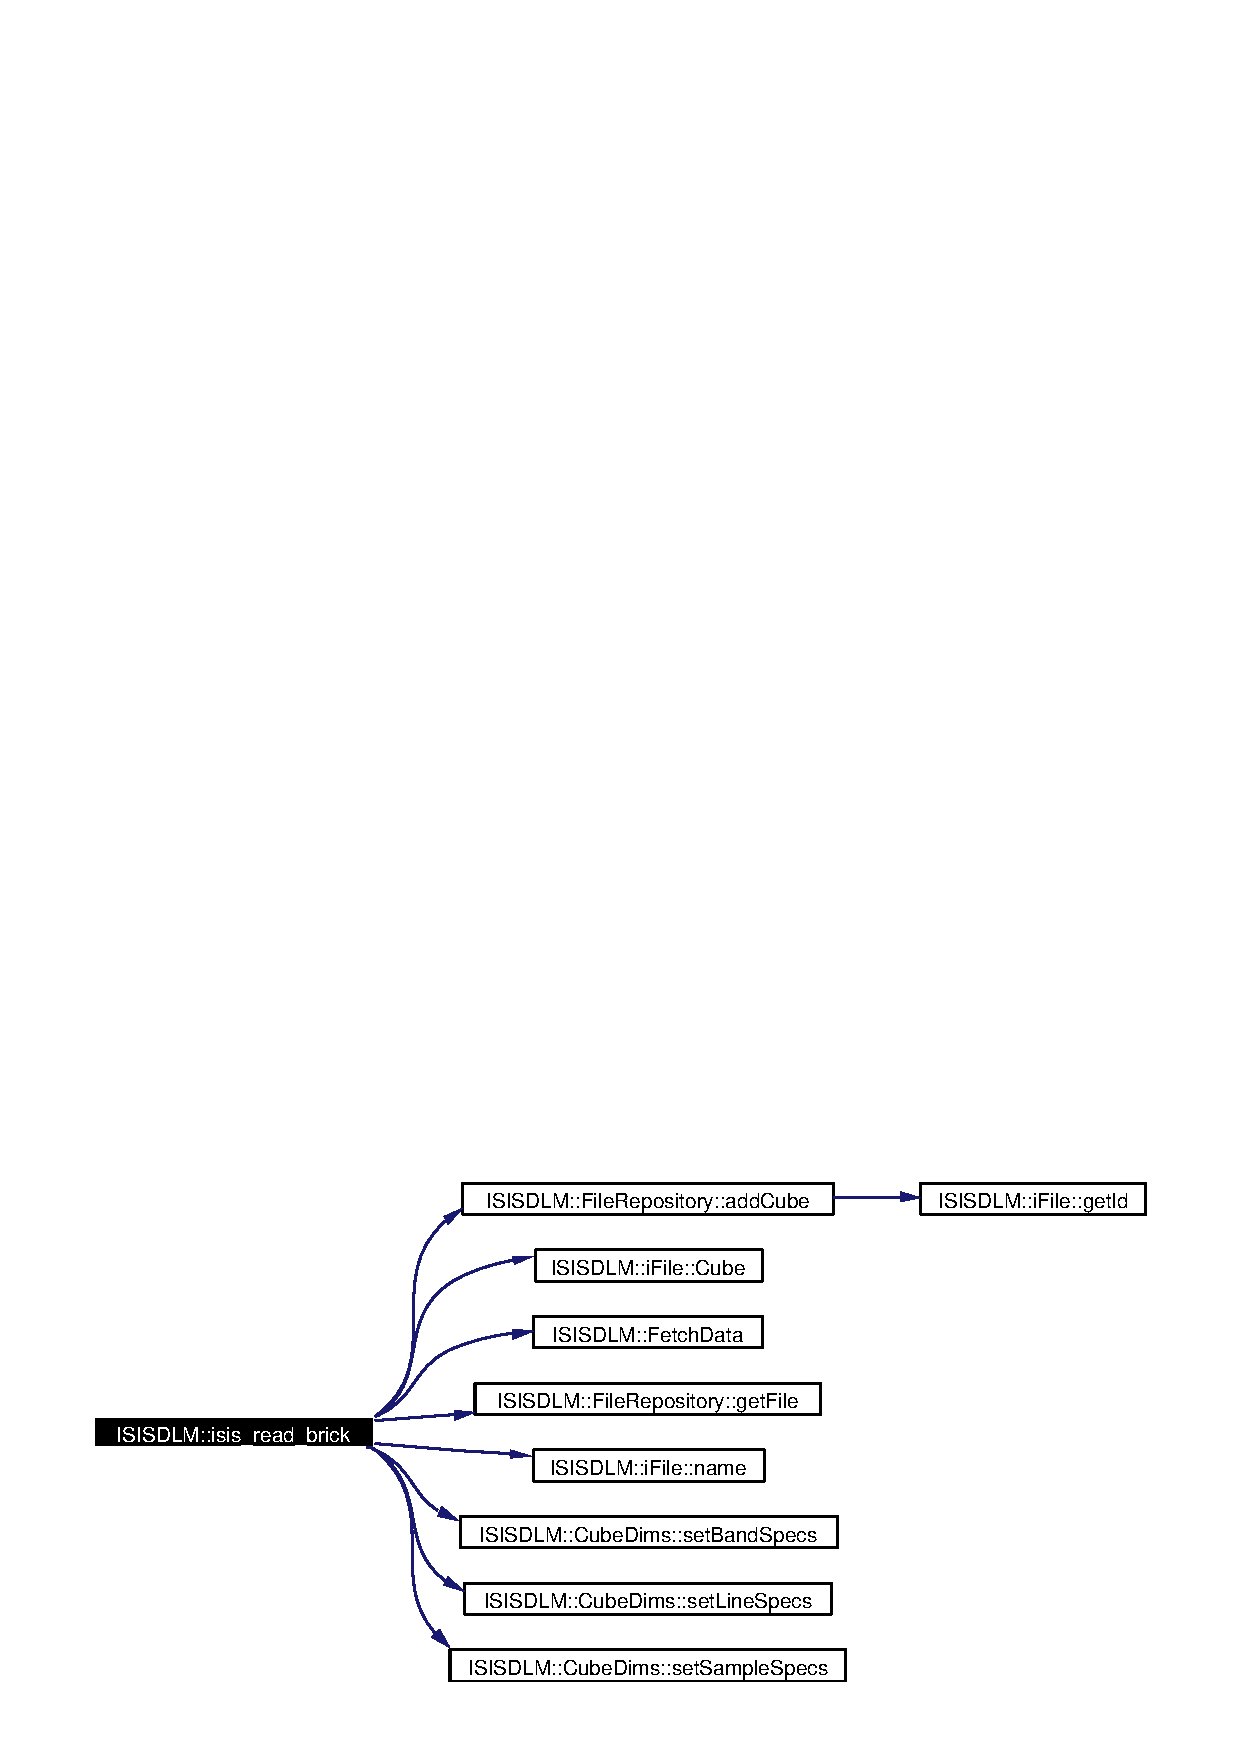
\includegraphics[width=279pt]{namespaceISISDLM_a31_cgraph}
\end{center}
\end{figure}
\index{ISISDLM@{ISISDLM}!isis_read_brick_init@{isis\_\-read\_\-brick\_\-init}}
\index{isis_read_brick_init@{isis\_\-read\_\-brick\_\-init}!ISISDLM@{ISISDLM}}
\subsubsection{\setlength{\rightskip}{0pt plus 5cm}int isis\_\-read\_\-brick\_\-init (Idl\-Dlm \& {\em idl})}\label{namespaceISISDLM_a30}


Performs initialization of isis\_\-read\_\-brick routine The isis\_\-read\_\-brick\_\-init function defines the isis\_\-read\_\-brick routine and registers it to the {\bf IDL} DLM toolkit. \begin{Desc}
\item[Parameters:]
\begin{description}
\item[{\em idl}]{\bf IDL} DLM interface \end{description}
\end{Desc}
\begin{Desc}
\item[Returns:]0 if successful, 1 otherwise \end{Desc}


Here is the call graph for this function:\begin{figure}[H]
\begin{center}
\leavevmode
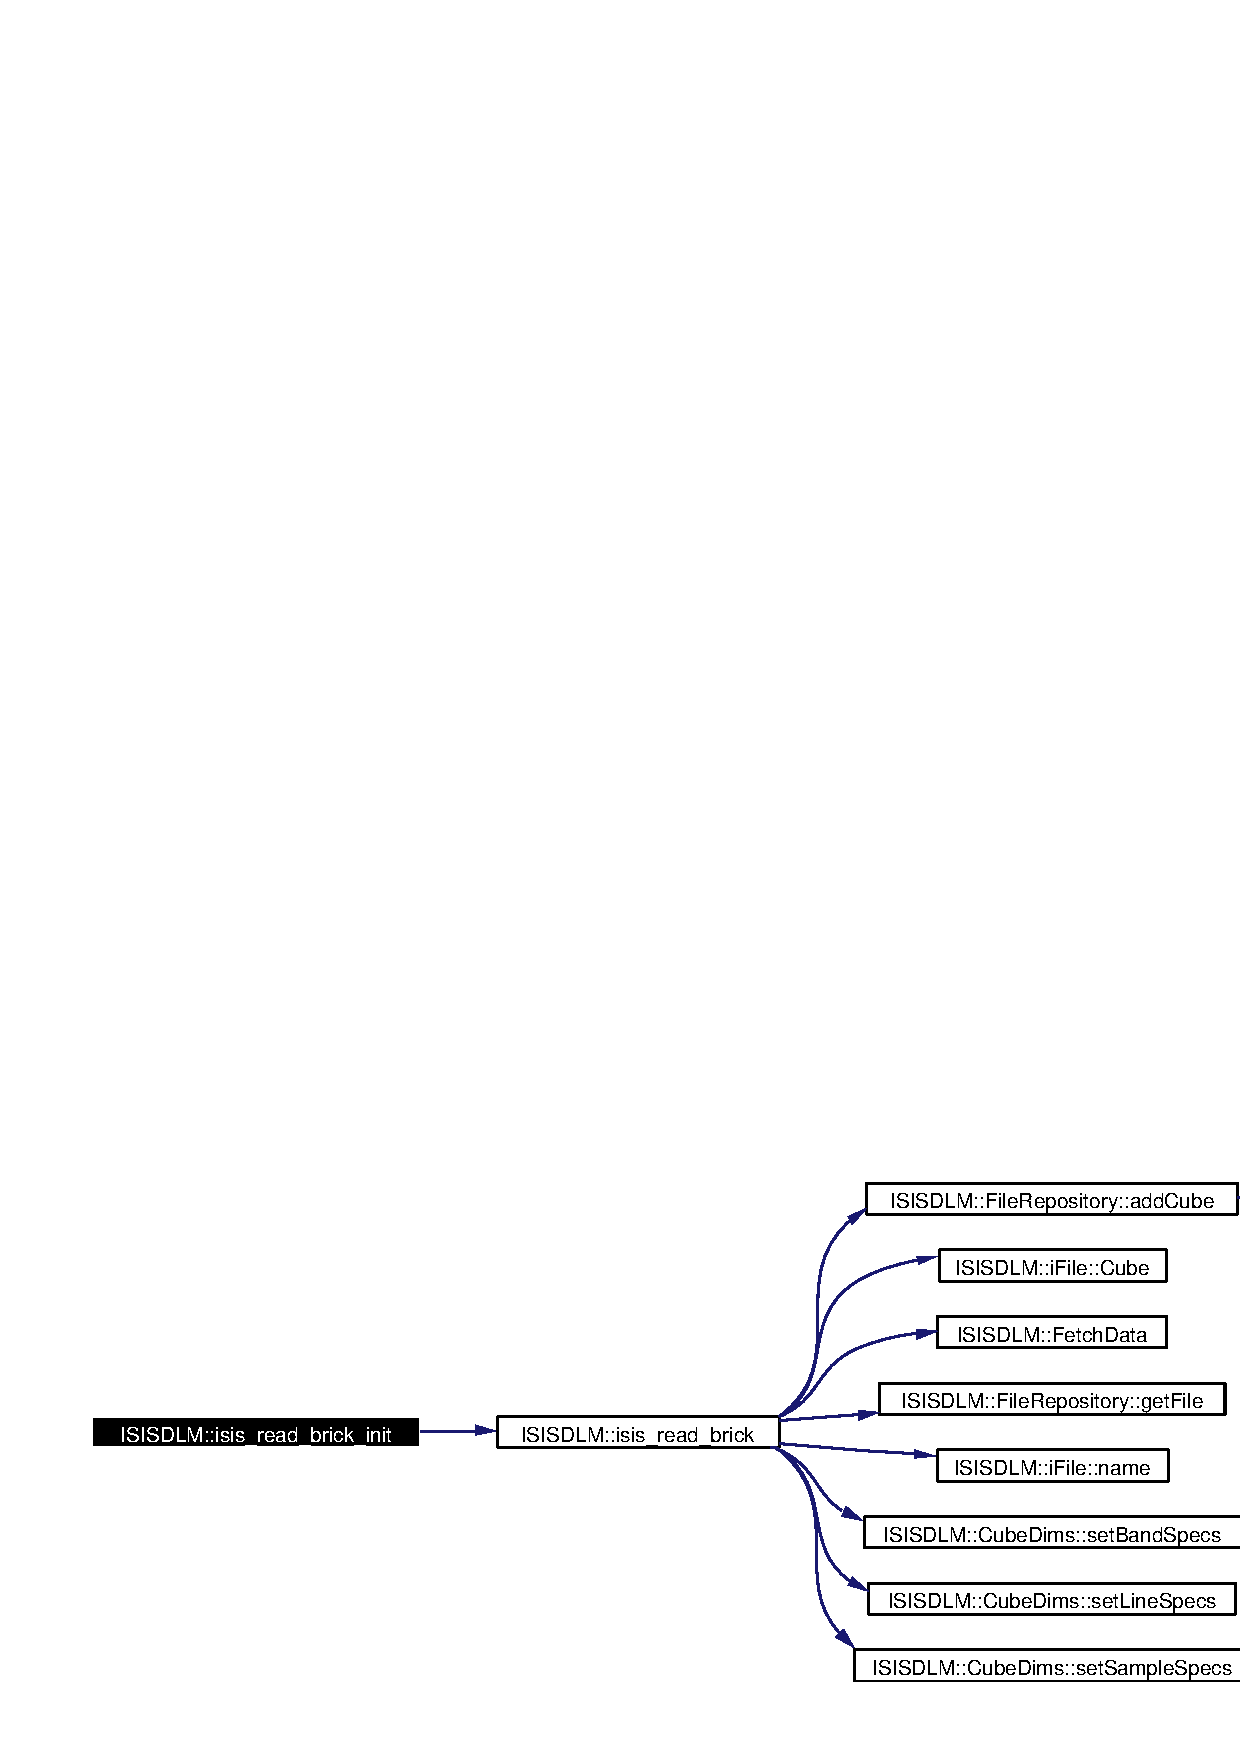
\includegraphics[width=376pt]{namespaceISISDLM_a30_cgraph}
\end{center}
\end{figure}
\index{ISISDLM@{ISISDLM}!isis_read_image@{isis\_\-read\_\-image}}
\index{isis_read_image@{isis\_\-read\_\-image}!ISISDLM@{ISISDLM}}
\subsubsection{\setlength{\rightskip}{0pt plus 5cm}int isis\_\-read\_\-image (const Idl\-Rtn\-Def \& {\em rtn}, const Idl\-Parameters \& {\em input}, Idl\-Parameters \& {\em output})}\label{namespaceISISDLM_a33}


Performs initialization of isis\_\-read\_\-image routine \begin{Desc}
\item[Parameters:]
\begin{description}
\item[{\em rtn}]Provides the function definition as specified in isis\_\-read\_\-image\_\-init \item[{\em input}]Contains a list of the input parameters \item[{\em output}]Will receive the parameters being passed back to {\bf IDL} user \end{description}
\end{Desc}
\begin{Desc}
\item[Returns:]0 if successful, 1 otherwise \end{Desc}


Here is the call graph for this function:\begin{figure}[H]
\begin{center}
\leavevmode
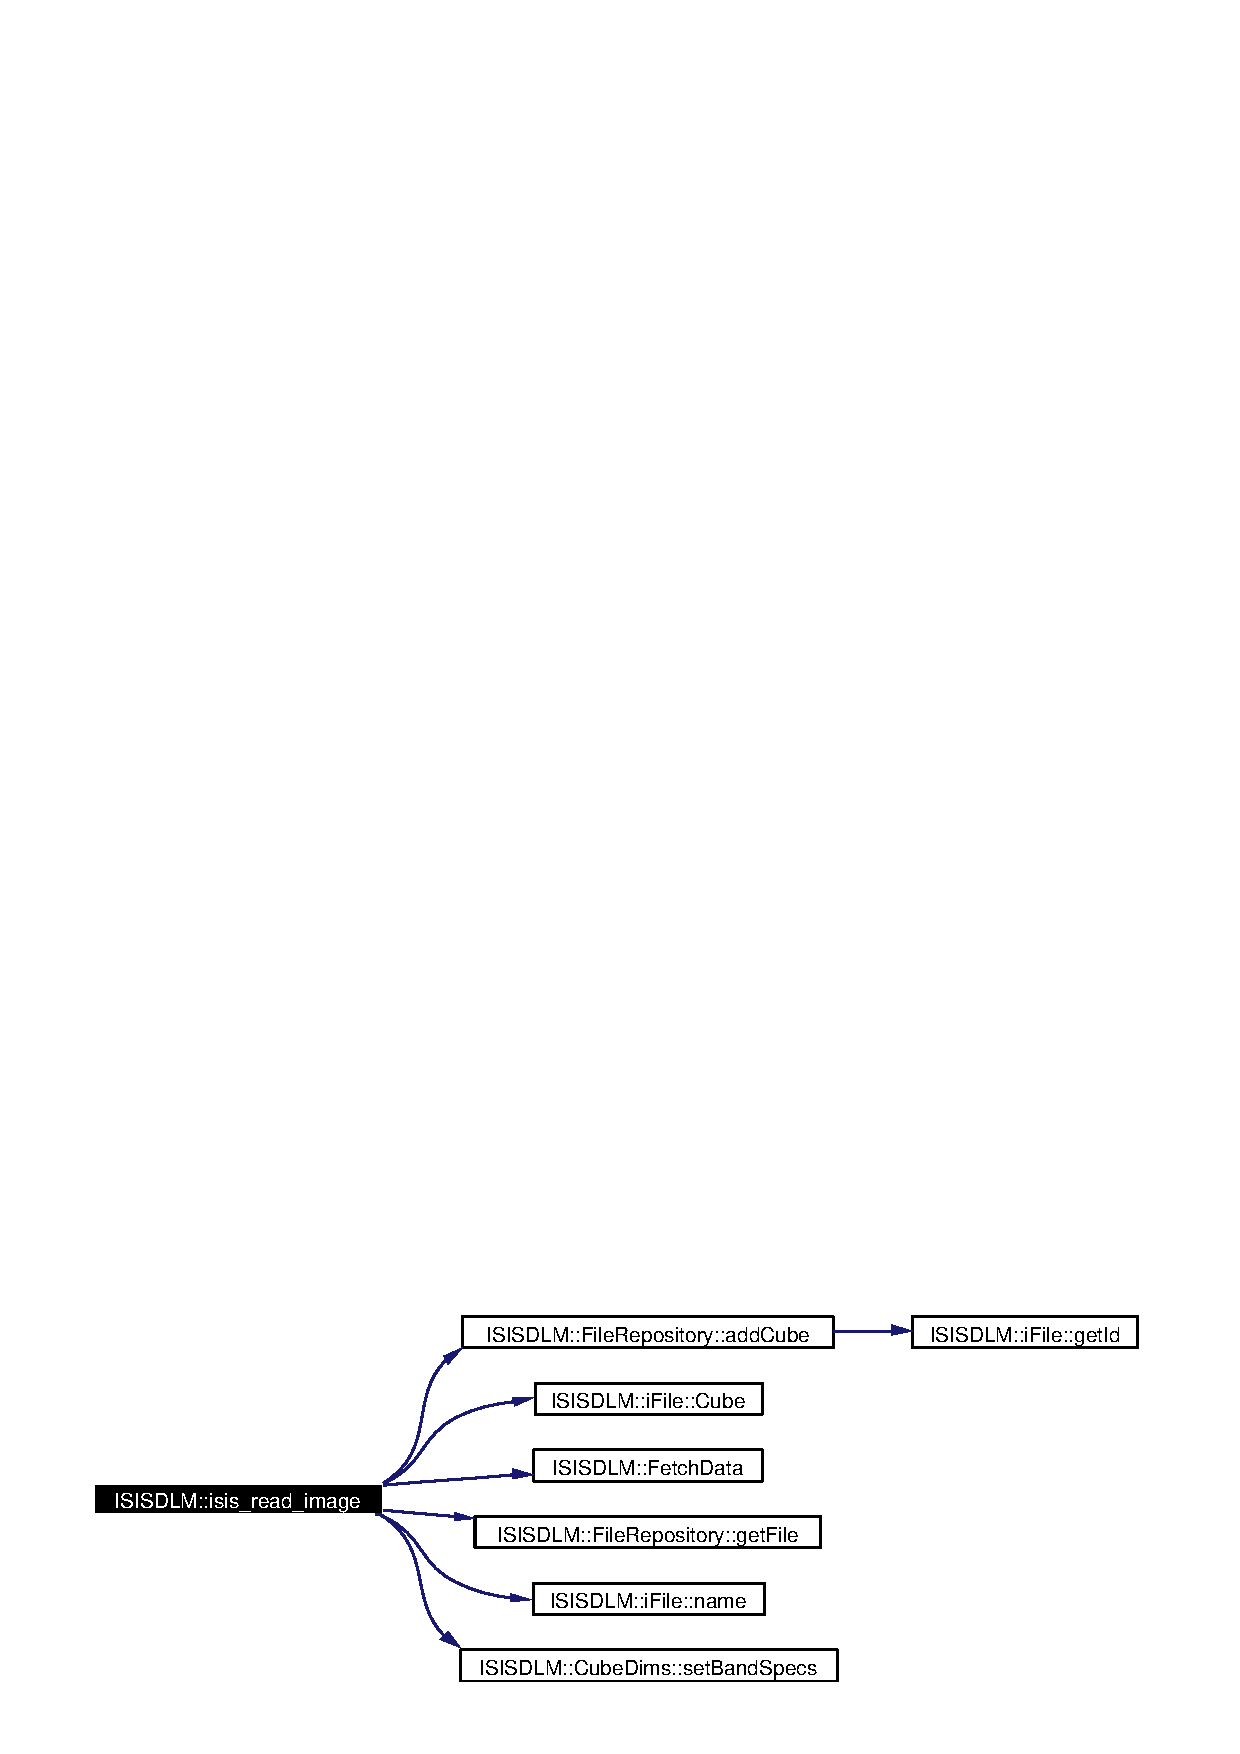
\includegraphics[width=277pt]{namespaceISISDLM_a33_cgraph}
\end{center}
\end{figure}
\index{ISISDLM@{ISISDLM}!isis_read_image_init@{isis\_\-read\_\-image\_\-init}}
\index{isis_read_image_init@{isis\_\-read\_\-image\_\-init}!ISISDLM@{ISISDLM}}
\subsubsection{\setlength{\rightskip}{0pt plus 5cm}int isis\_\-read\_\-image\_\-init (Idl\-Dlm \& {\em idl})}\label{namespaceISISDLM_a32}


Performs initialization of isis\_\-read\_\-image routine The isis\_\-read\_\-image\_\-init function defines the isis\_\-read\_\-image routine and registers it to the {\bf IDL} DLM toolkit. \begin{Desc}
\item[Parameters:]
\begin{description}
\item[{\em idl}]{\bf IDL} DLM interface \end{description}
\end{Desc}
\begin{Desc}
\item[Returns:]0 if successful, 1 otherwise \end{Desc}


Here is the call graph for this function:\begin{figure}[H]
\begin{center}
\leavevmode
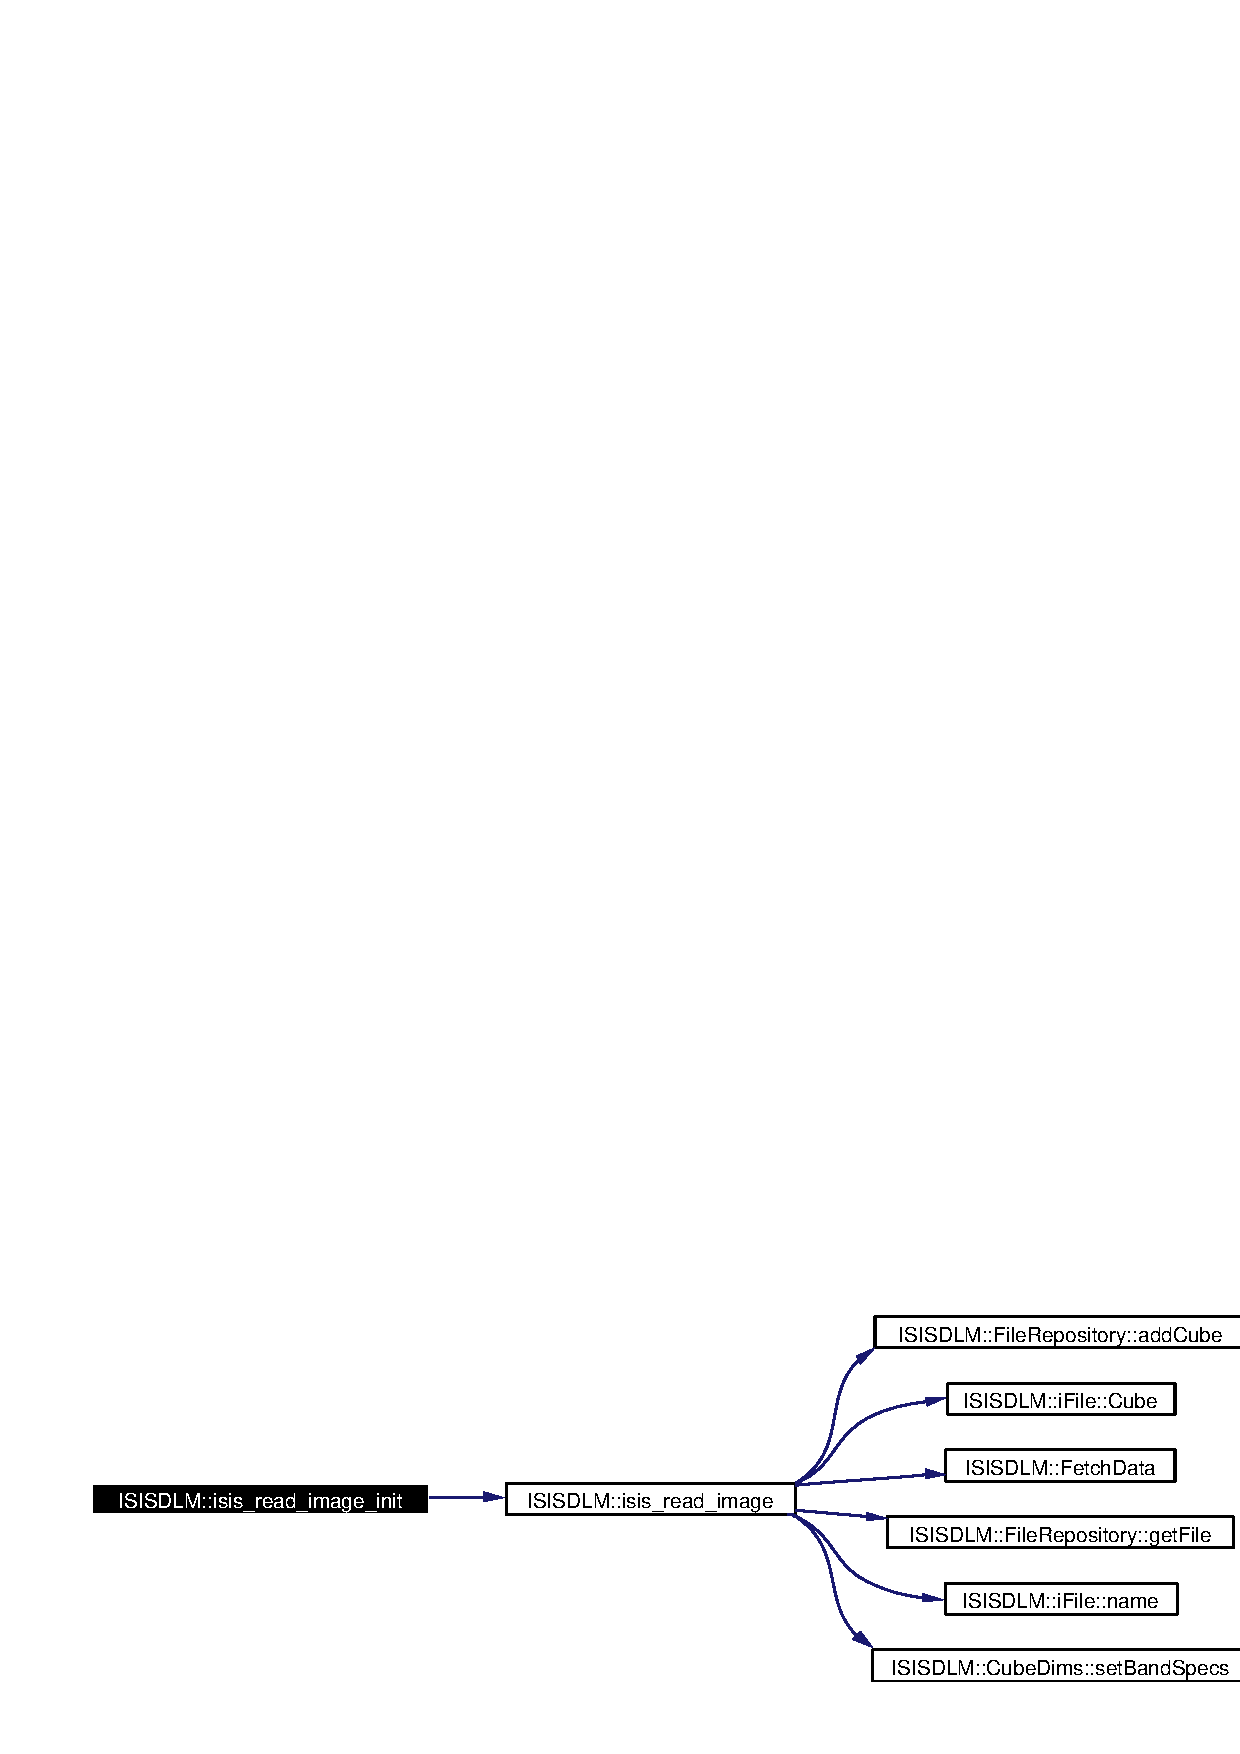
\includegraphics[width=376pt]{namespaceISISDLM_a32_cgraph}
\end{center}
\end{figure}
\index{ISISDLM@{ISISDLM}!isis_read_init@{isis\_\-read\_\-init}}
\index{isis_read_init@{isis\_\-read\_\-init}!ISISDLM@{ISISDLM}}
\subsubsection{\setlength{\rightskip}{0pt plus 5cm}int isis\_\-read\_\-init (Idl\-Dlm \& {\em idl})}\label{namespaceISISDLM_a26}


Performs initialization of isis\_\-read routine The isis\_\-read\_\-init function defines the isis\_\-read routine and registers it to the {\bf IDL} DLM toolkit. \begin{Desc}
\item[Parameters:]
\begin{description}
\item[{\em idl}]{\bf IDL} DLM interface \end{description}
\end{Desc}
\begin{Desc}
\item[Returns:]0 if successful, 1 otherwise \end{Desc}


Here is the call graph for this function:\begin{figure}[H]
\begin{center}
\leavevmode
\includegraphics[width=337pt]{namespaceISISDLM_a26_cgraph}
\end{center}
\end{figure}
\index{ISISDLM@{ISISDLM}!isis_special_pixels@{isis\_\-special\_\-pixels}}
\index{isis_special_pixels@{isis\_\-special\_\-pixels}!ISISDLM@{ISISDLM}}
\subsubsection{\setlength{\rightskip}{0pt plus 5cm}int isis\_\-special\_\-pixels (const Idl\-Rtn\-Def \& {\em rtn}, const Idl\-Parameters \& {\em input}, Idl\-Parameters \& {\em output})}\label{namespaceISISDLM_a35}


Performs initialization of isis\_\-special\_\-pixels routine \begin{Desc}
\item[Parameters:]
\begin{description}
\item[{\em rtn}]Provides the function definition as specified in isis\_\-special\_\-pixels\_\-init \item[{\em input}]Contains a list of the input parameters \item[{\em output}]Will receive the parameters being passed back to {\bf IDL} user \end{description}
\end{Desc}
\begin{Desc}
\item[Returns:]0 if successful, 1 otherwise \end{Desc}
\index{ISISDLM@{ISISDLM}!isis_special_pixels_init@{isis\_\-special\_\-pixels\_\-init}}
\index{isis_special_pixels_init@{isis\_\-special\_\-pixels\_\-init}!ISISDLM@{ISISDLM}}
\subsubsection{\setlength{\rightskip}{0pt plus 5cm}int isis\_\-special\_\-pixels\_\-init (Idl\-Dlm \& {\em idl})}\label{namespaceISISDLM_a34}


Performs initialization of isis\_\-special\_\-pixels routine The isis\_\-special\_\-pixels\_\-init function defines the isis\_\-special\_\-pixels routine and registers it to the {\bf IDL} DLM toolkit. \begin{Desc}
\item[Parameters:]
\begin{description}
\item[{\em idl}]{\bf IDL} DLM interface \end{description}
\end{Desc}
\begin{Desc}
\item[Returns:]0 if successful, 1 otherwise \end{Desc}


Here is the call graph for this function:\begin{figure}[H]
\begin{center}
\leavevmode
\includegraphics[width=204pt]{namespaceISISDLM_a34_cgraph}
\end{center}
\end{figure}
\index{ISISDLM@{ISISDLM}!isis_write@{isis\_\-write}}
\index{isis_write@{isis\_\-write}!ISISDLM@{ISISDLM}}
\subsubsection{\setlength{\rightskip}{0pt plus 5cm}int isis\_\-write (const Idl\-Rtn\-Def \& {\em rtn}, const Idl\-Parameters \& {\em input}, Idl\-Parameters \& {\em output})}\label{namespaceISISDLM_a37}


Performs initialization of isis\_\-write routine \begin{Desc}
\item[Parameters:]
\begin{description}
\item[{\em rtn}]Provides the function definition as specified in isis\_\-write\_\-init \item[{\em input}]Contains a list of the input parameters \item[{\em output}]Will receive the parameters being passed back to {\bf IDL} user \end{description}
\end{Desc}
\begin{Desc}
\item[Returns:]0 if successful, 1 otherwise \end{Desc}


Here is the call graph for this function:\begin{figure}[H]
\begin{center}
\leavevmode
\includegraphics[width=258pt]{namespaceISISDLM_a37_cgraph}
\end{center}
\end{figure}
\index{ISISDLM@{ISISDLM}!isis_write_image@{isis\_\-write\_\-image}}
\index{isis_write_image@{isis\_\-write\_\-image}!ISISDLM@{ISISDLM}}
\subsubsection{\setlength{\rightskip}{0pt plus 5cm}int isis\_\-write\_\-image (const Idl\-Rtn\-Def \& {\em rtn}, const Idl\-Parameters \& {\em input}, Idl\-Parameters \& {\em output})}\label{namespaceISISDLM_a39}


Performs initialization of isis\_\-write\_\-image routine \begin{Desc}
\item[Parameters:]
\begin{description}
\item[{\em rtn}]Provides the function definition as specified in isis\_\-write\_\-image\_\-init \item[{\em input}]Contains a list of the input parameters \item[{\em output}]Will receive the parameters being passed back to {\bf IDL} user \end{description}
\end{Desc}
\begin{Desc}
\item[Returns:]0 if successful, 1 otherwise \end{Desc}


Here is the call graph for this function:\begin{figure}[H]
\begin{center}
\leavevmode
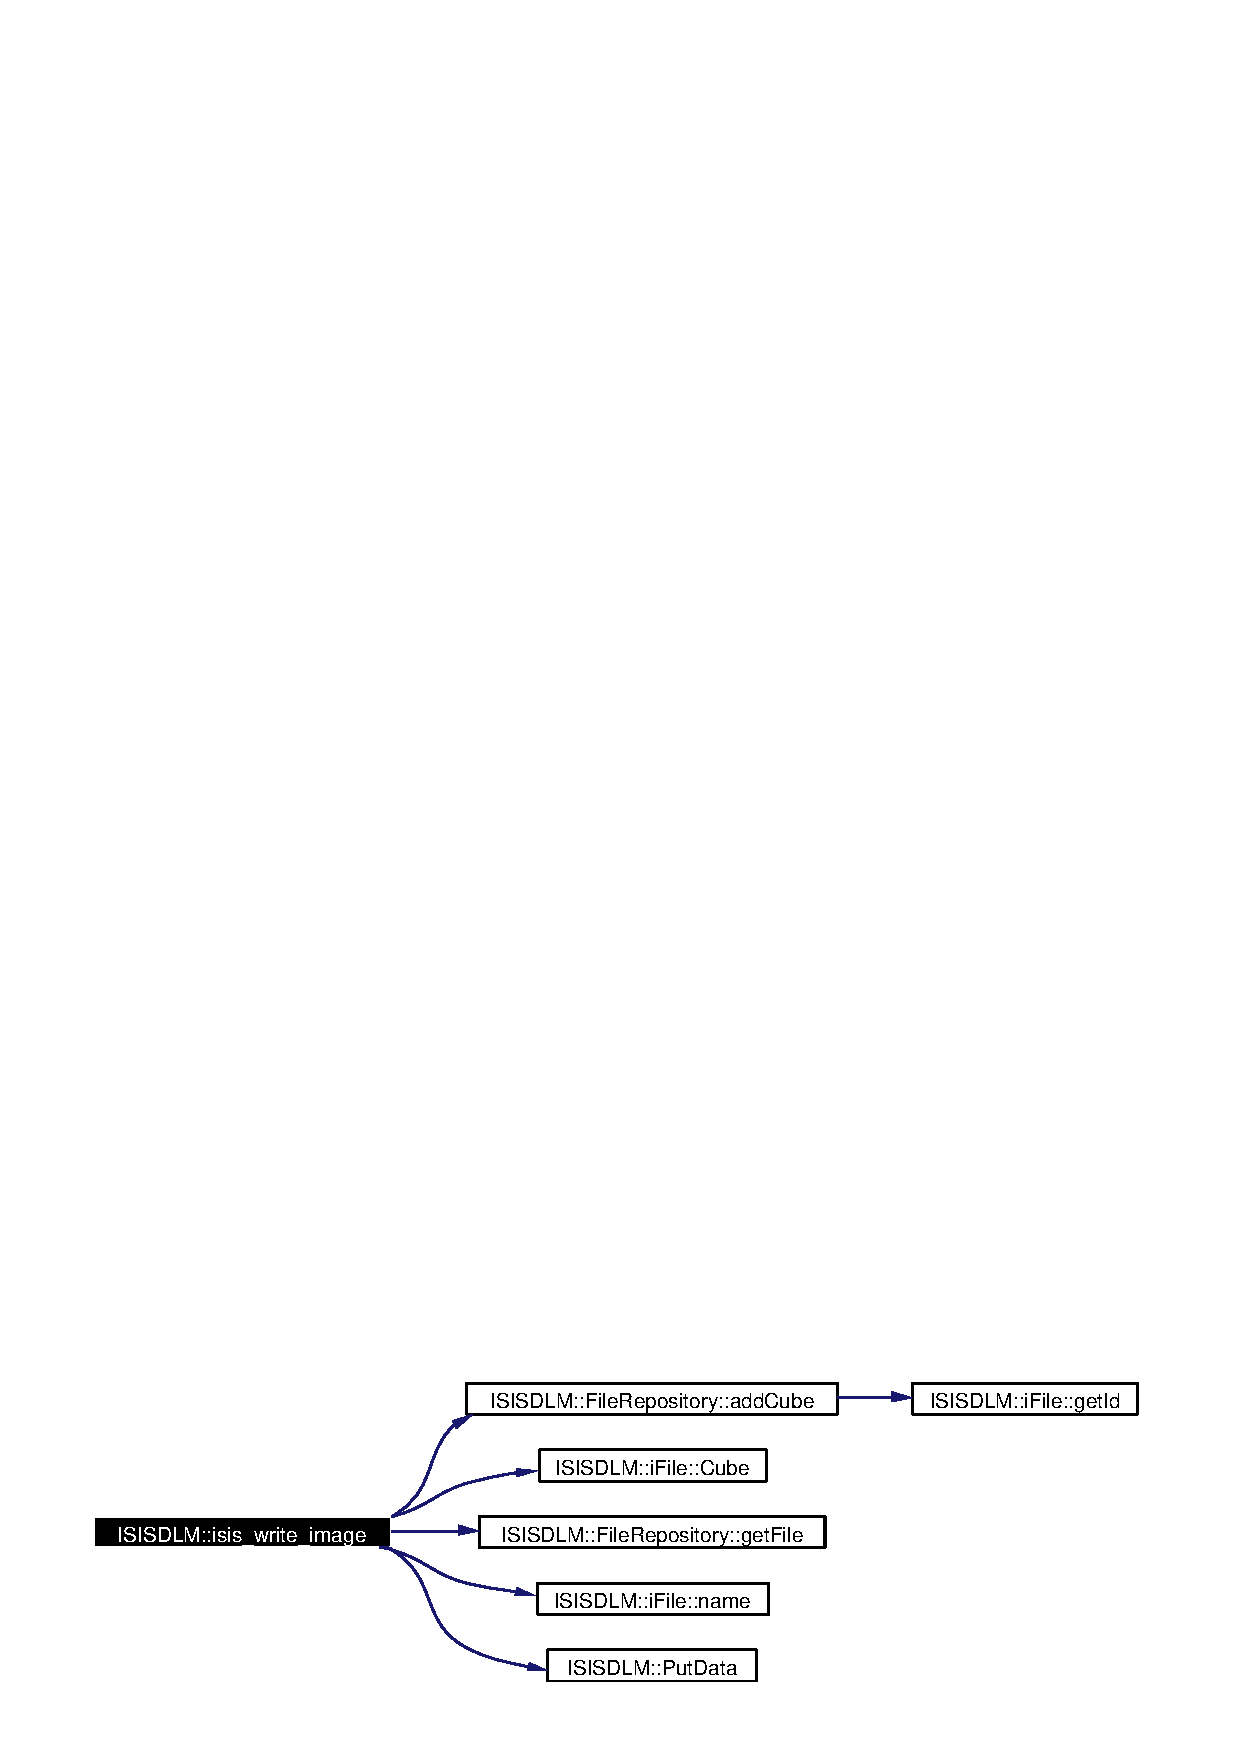
\includegraphics[width=277pt]{namespaceISISDLM_a39_cgraph}
\end{center}
\end{figure}
\index{ISISDLM@{ISISDLM}!isis_write_image_init@{isis\_\-write\_\-image\_\-init}}
\index{isis_write_image_init@{isis\_\-write\_\-image\_\-init}!ISISDLM@{ISISDLM}}
\subsubsection{\setlength{\rightskip}{0pt plus 5cm}int isis\_\-write\_\-image\_\-init (Idl\-Dlm \& {\em idl})}\label{namespaceISISDLM_a38}


Performs initialization of isis\_\-write\_\-image routine The isis\_\-write\_\-image\_\-init function defines the isis\_\-write\_\-image routine and registers it to the {\bf IDL} DLM toolkit. \begin{Desc}
\item[Parameters:]
\begin{description}
\item[{\em idl}]{\bf IDL} DLM interface \end{description}
\end{Desc}
\begin{Desc}
\item[Returns:]0 if successful, 1 otherwise \end{Desc}


Here is the call graph for this function:\begin{figure}[H]
\begin{center}
\leavevmode
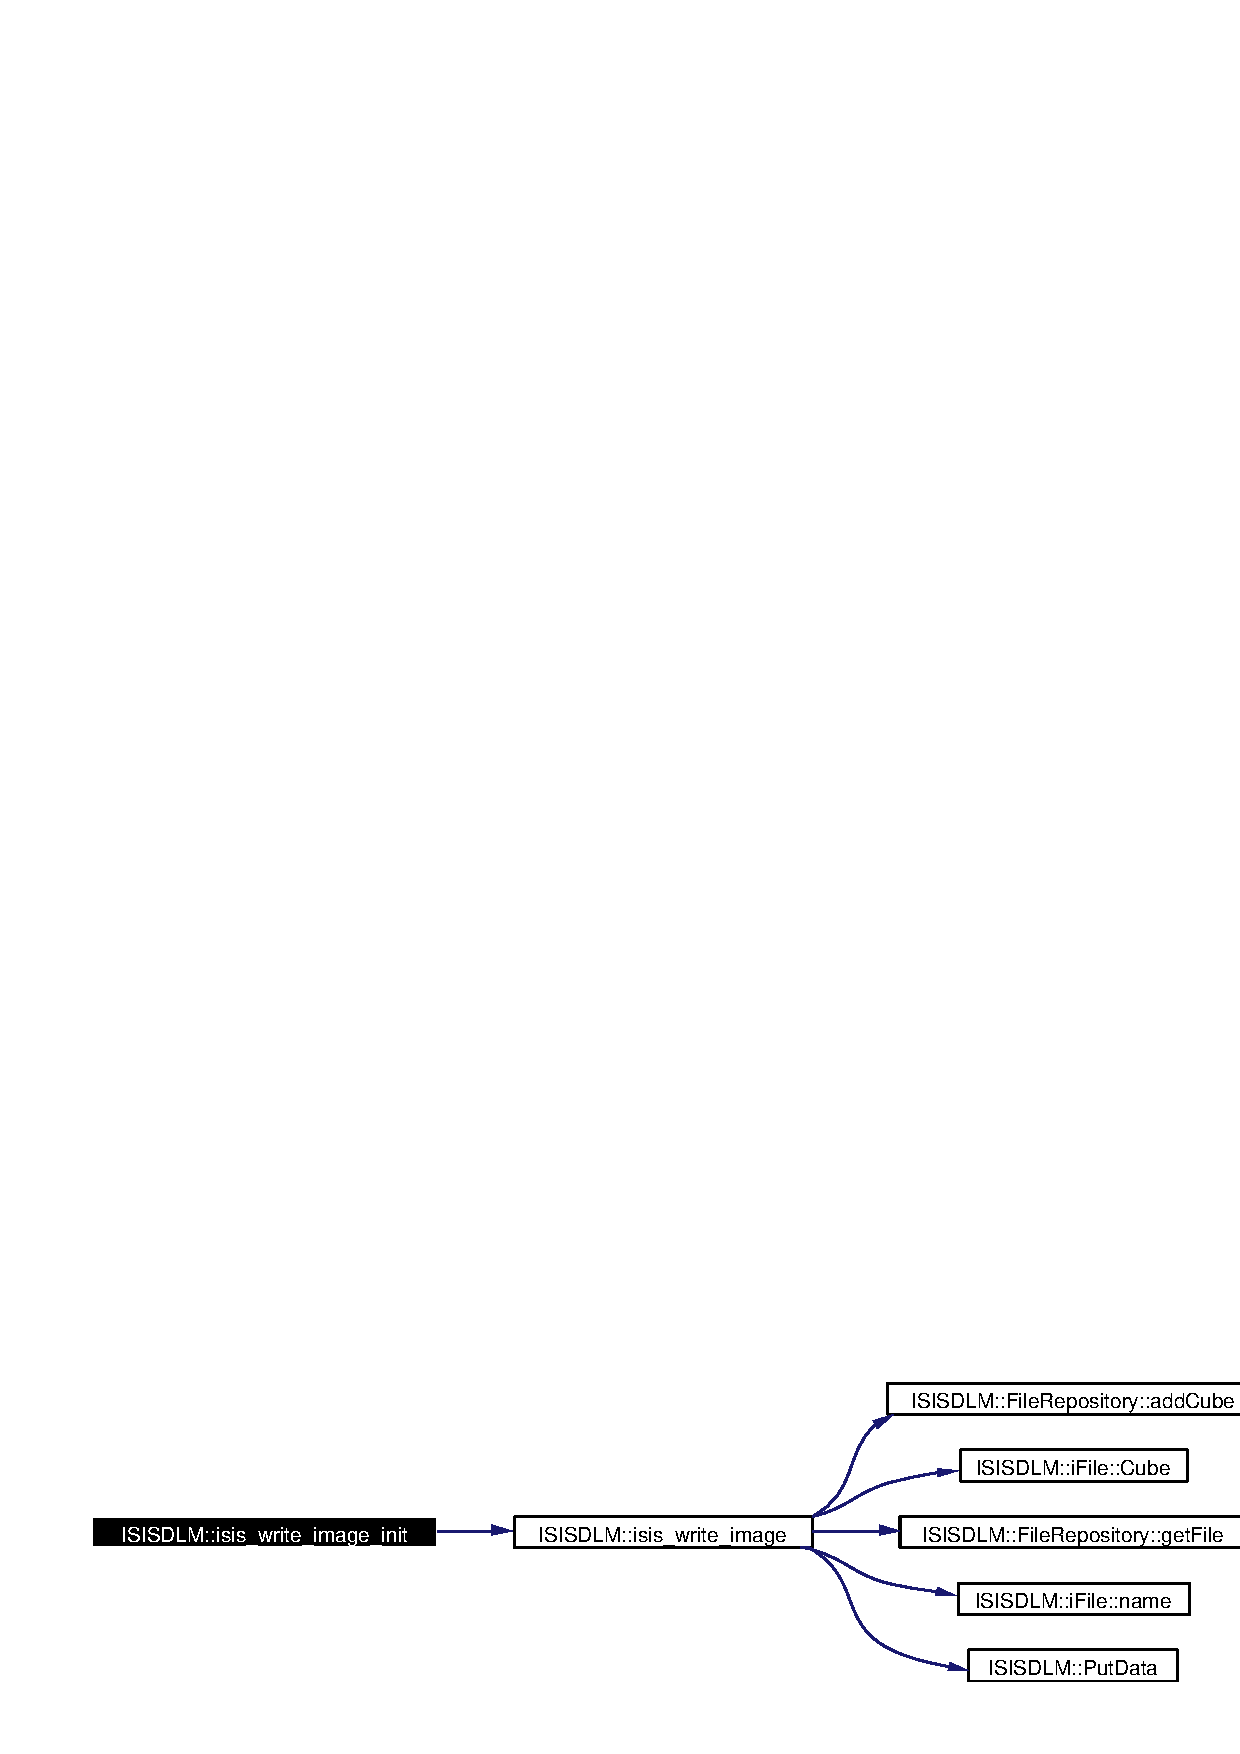
\includegraphics[width=378pt]{namespaceISISDLM_a38_cgraph}
\end{center}
\end{figure}
\index{ISISDLM@{ISISDLM}!isis_write_init@{isis\_\-write\_\-init}}
\index{isis_write_init@{isis\_\-write\_\-init}!ISISDLM@{ISISDLM}}
\subsubsection{\setlength{\rightskip}{0pt plus 5cm}int isis\_\-write\_\-init (Idl\-Dlm \& {\em idl})}\label{namespaceISISDLM_a36}


Performs initialization of isis\_\-write routine The isis\_\-write\_\-init function defines the isis\_\-write routine and registers it to the {\bf IDL} DLM toolkit. \begin{Desc}
\item[Parameters:]
\begin{description}
\item[{\em idl}]{\bf IDL} DLM interface \end{description}
\end{Desc}
\begin{Desc}
\item[Returns:]0 if successful, 1 otherwise \end{Desc}


Here is the call graph for this function:\begin{figure}[H]
\begin{center}
\leavevmode
\includegraphics[width=341pt]{namespaceISISDLM_a36_cgraph}
\end{center}
\end{figure}
\index{ISISDLM@{ISISDLM}!PutData@{PutData}}
\index{PutData@{PutData}!ISISDLM@{ISISDLM}}
\subsubsection{\setlength{\rightskip}{0pt plus 5cm}template$<$class T$>$ void Put\-Data (T \& {\em writer}, Isis::Cube \& {\em cube}, const IDL::Array\-Dims \& {\em dims}, IDL::Idl\-Variable \& {\em v\-Data})}\label{namespaceISISDLM_a6}


The write routine that interfaces with the ISIS I/O engines This routine is used to read all kinds of data types \index{ISISDLM@{ISISDLM}!show_file_data@{show\_\-file\_\-data}}
\index{show_file_data@{show\_\-file\_\-data}!ISISDLM@{ISISDLM}}
\subsubsection{\setlength{\rightskip}{0pt plus 5cm}void show\_\-file\_\-data (const Idl\-Rtn\-Def \& {\em rtn}, i\-File \& {\em file})}\label{namespaceISISDLM_a22}




Here is the call graph for this function:\begin{figure}[H]
\begin{center}
\leavevmode
\includegraphics[width=169pt]{namespaceISISDLM_a22_cgraph}
\end{center}
\end{figure}
